\documentclass[10pt,a4paper]{amsart}
\usepackage{amsmath,amssymb,amsthm,graphicx}
\usepackage[no-math]{fontspec}
\setmainfont{DejaVu Serif}
\usepackage{mathtools,proof,tikz,csquotes,needspace,enumerate,xspace,array,xcolor}
\newcommand{\faBible}{\raisebox{-0.1254em}{
\includegraphics[height=1em]{author-bible-glyph.pdf}}}
\usepackage{hyperref}
\usepackage[capitalise]{cleveref}
\usetikzlibrary{calc,positioning}
\definecolor{lipicsYellow}{RGB}{255,204,0}
\definecolor{lipicsGray}{gray}{0.4}
\tikzstyle{m}=[fill=white,inner sep=1,scale=0.75]
\tikzstyle{n}=[fill=lipicsYellow!50,inner sep=1,rounded corners]
\tikzstyle{b}=[lipicsGray,thick]
\newtheorem{theorem}{Theorem}
\newtheorem{lemma}[theorem]{Lemma}
\newtheorem{proposition}[theorem]{Proposition}
\newtheorem{corollary}[theorem]{Corollary}
\theoremstyle{definition}
\newtheorem{definition}[theorem]{Definition}
\newtheorem{example}[theorem]{Example}
\newtheorem{remark}[theorem]{Remark}
\newtheorem{notation}[theorem]{Notation}
\newtheorem{problem}[theorem]{Problem}
\providecommand{\todo}[2][]{}
% BEGIN unchanged author macros.tex
% !TEX root = CerdaMS.tex

% ========== Comments macros ==========

\newcommand{\comas}	[1]	{\todo[color=cyan]			{Alex: #1}}
\newcommand{\comasi}[1]	{\todo[color=cyan,inline]	{Alex: #1}}
\newcommand{\comrc}	[1]	{\todo[color=orange]		{Rémy: #1}}
\newcommand{\comrci}[1]	{\todo[color=orange,inline]	{Rémy: #1}}
\newcommand{\comgm}	[1]	{\todo[color=green]			{Giulio: #1}}
\newcommand{\comgmi}[1]	{\todo[color=green,inline]	{Giulio: #1}}


% ========== Text macros ==========

\newcommand{\bsub}{\begin{enumerate}[(i)]}
\newcommand{\esub}{\end{enumerate}}

\NewDocumentCommand \lam		{}		
	{\texorpdfstring{\ensuremath{\lambda}}{lambda}}
\NewDocumentCommand \lamI		{}		
	{\texorpdfstring{\ensuremath{\lambda\comb{I}}}{lambda-I}}
\NewDocumentCommand \lamK		{}		
	{\texorpdfstring{\ensuremath{\lambda\comb{K}}}{lambda-K}}

% Emphasizing defined terms
\NewDocumentCommand \defemph 	{m} 	{\emph{#1}}


% ========== Basic stuff ==========

% Defining objects

\NewDocumentCommand \eqdef		{}		{ \coloneqq }
\NewDocumentCommand \eqbnf		{}		{ \mathrel{\Coloneqq} }
\NewDocumentCommand \eqcobnf	{}		
	{ \mathrel{\Coloneqq}_{\textrm{co-ind.}} }
\NewDocumentCommand \bnf		{ommo}
	{\[	\IfValueT{#1}{#1 \quad \ni \quad}
		#2 \eqbnf #3
		\IfValueT{#4}{\quad (#4)}
	\]}
\NewDocumentCommand \cobnf		{ommo}
	{\[	\IfValueT{#1}{#1 \quad \ni \quad}
		#2 \eqcobnf #3
		\IfValueT{#4}{\quad (#4)}
	\]}

% Set theory

\NewDocumentCommand \set 		{smo}	
	{\IfBooleanTF{#1}
		{ \left\{ #2 \IfValueT{#3}{ \ \middle|\ #3 } \right\} }
		{ \{ #2 \IfValueT{#3}{ \ |\ #3 } \} }
	}

\NewDocumentCommand \subf		{}		{ \subseteq_{\mathrm{f}} }
\RenewDocumentCommand \emptyset {}		{ \varnothing }
\RenewDocumentCommand \setminus {}		{ - }
\NewDocumentCommand	\parts		{m}		{ \cramped{2^{#1}} }
\NewDocumentCommand \bigdunion	{}		{ \coprod }

% Predefined sets

\NewDocumentCommand \Nat 		{}		{ \mathbb{N} }
\NewDocumentCommand \Var		{}		{ \mathcal{V} }

% Rewriting

\NewDocumentCommand \red 			{oo}	
	{ \rightarrow \IfValueTF{#1}
		{ \IfValueTF{#2}{ _{#1}^{#2} }{ _{#1} } }
		{ \IfValueT{#2}{ ^{#2} } } 
	}
\NewDocumentCommand \redd 			{oo}	
	{ \mathrel{\rightarrow\mathrel{\mkern-14mu}\rightarrow} \IfValueTF{#1}
		{ \IfValueTF{#2}{ _{#1}^{#2} }{ _{#1} } }
		{ \IfValueT{#2}{ ^{#2} } } 
	}


% ========== λ(I)-calculus ==========


% Sets of λ-terms
\NewDocumentCommand \Lam		{}		{ \Lambda }
\NewDocumentCommand \LamI		{}		{ \Lambda_\comb{I} }

\NewDocumentCommand \subst 		{om}	
	{[ #2 / \IfValueTF{#1}{#1}{x}] }

% Combinators
\NewDocumentCommand \comb		{m}		{ \mathsf{#1} }
\NewDocumentCommand \Om			{}		{ \comb{\Omega} }
\NewDocumentCommand \Bible 		{o} 		
	{ \text{\scalebox{0.8}{\faBible}}_{\,\IfValueTF{#1}{#1}{l}} }

% \ensuremath{\beta}-reduction
\NewDocumentCommand \bred 		{} 		{ \red[\ensuremath{\beta}] }
\NewDocumentCommand \breds 		{} 		{ \redd[\ensuremath{\beta}] }


% ========== Resource calculus ==========

% Sets of resource expressions
\NewDocumentCommand \rterms		{ss}
	{\mathord{
		\IfBooleanTF{#1}{ \IfBooleanTF{#2}{(!)}{!} }{}
		\Delta_{\comb{I}}
	}}

% Sets of finite sums of resource expressions
\NewDocumentCommand \frsums 	{oss}
	{ \IfBooleanTF{#2}
		{ \IfBooleanTF{#3}
			{ \Nat[ \rterms** \IfValueT{#1}{(#1)} ] }
			{ \Nat[ \rterms* \IfValueT{#1}{(#1)} ] } }
		{ \Nat[ \rterms \IfValueT{#1}{(#1)} ] }
	}

% Empty sum
\NewDocumentCommand \esum		{m}		{ \rs{0}_{#1} }

% Formatting resource terms, bags, sums, and sums of bags
\NewDocumentCommand \rt			{m}		{ #1 }
\NewDocumentCommand \rb			{m}		{ \bar{#1} }
\NewDocumentCommand \rs			{m}		{ \mathbf{#1} }
\NewDocumentCommand \rbs		{m}		{ \bar{\mathbf{#1}} }

% Memory substitution
\NewDocumentCommand \msubst 	{mo}	
	{ \left\lbrace #1 \middle/ \IfValueTF{#2}{#2}{x} \right\rbrace }

% Resource substitution
\NewDocumentCommand \rsubst 	{smo}	
	{ \left\langle \IfBooleanTF{#1}{ #2 }{ \rb{#2} } \middle/ 
	\IfValueTF{#3}{ #3 }{ x } \right\rangle }

% Resource reduction
\NewDocumentCommand \resource	{}		{ \mathsf{r} }
\NewDocumentCommand \rred 		{} 		{ \red[\resource] }
\NewDocumentCommand \rredr 		{} 		{ \red[\resource][?] }
\NewDocumentCommand \rreds 		{} 		{ \redd[\resource] }

\NewDocumentCommand \nf 		{}		{ \mathrm{nf} }
\NewDocumentCommand \size		{m}		{ \mathsf{size}(#1) }
\NewDocumentCommand \sumsize	{m}		{ \mathsf{ssize}(#1) }

\NewDocumentCommand \supp		{sm}
	{ | \IfBooleanTF{#1}{#2}{\rs{#2}} | }

% Multiset ordering

\NewDocumentCommand \msetlt		{}		{ \prec_\Nat }
\NewDocumentCommand \msetgt		{}		{ \succ_\Nat }


% ========== Böhm-like trees and approximations ==========

\NewDocumentCommand \memory		{}		{ \mathsf{m} }

\NewDocumentCommand \fv 		{}		{ \mathrm{fv} }
\NewDocumentCommand \pfv 		{}		{ \mathrm{pfv} }

% Trees

\NewDocumentCommand \BT 		{m}		{ \mathrm{BT}(#1) }
\NewDocumentCommand \MT			{om}	
	{ \mathrm{OT}\IfValueT{#1}{^{#1}}(#2) }
\NewDocumentCommand \MTrees		{}		{ \mathcal{OT} }

\NewDocumentCommand \Appset		{}		{ \mathcal{A}_\memory }
\NewDocumentCommand \Appof		{m}		{ \mathrm{App}_\memory(#1) }
\NewDocumentCommand \dirapp		{m}		{ \omega_\memory(#1) }
\NewDocumentCommand \MTle		{}		{ \sqsubseteq }
\NewDocumentCommand \MTlub		{}		{ \sqcup }
\NewDocumentCommand \bigMTlub	{}		{ \bigsqcup }

% The bijection Ohana trees ↔ Sets of approximants
\NewDocumentCommand \mtapp		{m}		{ {\cal A}(#1) }
\NewDocumentCommand \appmt		{m}		{ {\cal T}(#1) }

% Taylor

\NewDocumentCommand \TE 		{ssm}	
	{ \mathcal{T}_\memory^{
		\IfBooleanT{#1}{\IfBooleanTF{#2}{!}{\bullet}}
	} (#3) }
\NewDocumentCommand \TMT		{ssm}
	{ \IfBooleanTF{#1}
		{ \IfBooleanTF{#2}{ \TE**{\MT{#3}} }{ \TE*{\MT{#3}} } }
		{ \TE{\MT{#3}} } 
	}
\NewDocumentCommand \NFT		{ssm}
	{ \nf( \IfBooleanTF{#1}
		{ \IfBooleanTF{#2}{ \TE**{#3} }{ \TE*{#3} } }
		{ \TE{#3} } 
	) }

\NewDocumentCommand \TEin		{}		{ \in^\bullet }
\NewDocumentCommand \TElt		{}		{ \subseteq^\bullet }
\NewDocumentCommand \TElub		{}		{ \cup^\bullet }
\NewDocumentCommand \bigTElub	{}			
	{ \mathop{\bigcup\nolimits^{\mathrlap{\bullet}}}\displaylimits }

\NewDocumentCommand \resourceof	{sm}	
	{ [\![#2]\!]_\resource^{\IfBooleanT{#1}{!}} }

% Associated theories

\NewDocumentCommand \cB			{}		{ \mathcal{B} }
\NewDocumentCommand \cT			{}		{ \mathcal{T} }
\NewDocumentCommand \cM			{}		{ \mathcal{O} }
\NewDocumentCommand \cX			{}		{ \mathcal{X} }
\NewDocumentCommand \cY			{}		{ \mathcal{Y} }
\NewDocumentCommand \model		{m}		{ \mathcal{#1} } 
% find a font for models


% END unchanged author macros.tex

\providecommand{\cal}{\mathcal}
\title{Taylor expansion with memory commutes with Ohana trees in the lambda-I calculus}
\author{Rémy Cerda, Giulio Manzonetto, Alexis Saurin}
\date{doi:10.4230/LIPIcs.FSCD.2025.12; CC BY4.0 (publisher and linked arXiv2505.06193v2)}
\begin{document}
\maketitle
\noindent\textit{Editorial note.} Source https://drops.dagstuhl.de/entities/document/10.4230/LIPIcs.FSCD.2025.12 and its linked arXiv2505.06193v2 conference version with complete proof appendices, CC BY4.0. Author native mathematical TeX and figure macros retained unchanged.\par\medskip
\noindent\textit{Allowed standard prerequisites (editorial).}\begin{itemize}
\item Standard lambda-calculus head reduction, Church-Rosser and λI normalization properties. Author §2 and reference Barendregt; complete source bibliography retained. Resource/Ohana-specific proofs are included rather than treated as background.
\end{itemize}\medskip
% !TEX root = ../CerdaMS.tex

\section{Preliminaries}

We recall some basic notions and results concerning the \lam-calculus, and its fragment without weakening known as the \lamI-calculus. For more information, we refer to Barendregt's book \cite{Bare}.

\subsection{The \lam-calculus, in a nutshell} 
Let us fix an infinite set $\Var$ of variables. The set $\Lam$ of 
\emph{\lam-terms} is defined by induction
\bnf[\Lam]{M,N}{ x \mid \lam x.M \mid MN }[\text{for $x \in \Var$}]
We use parentheses when needed.
We assume that application associates on the left, 
and has higher precedence than abstraction.
E.g., $\lam x.\lam y.\lam z.xyz$ stands for $\lam x.(\lam y.(\lam z.(xy)z))$.
We write $\lam x_1 \ldots x_n.M$ or even $\lam\vec x.M$ 
for $\lam x_1.\ldots \lam x_n.M$, 
and $N^n(M)$ for $N(N(\cdots N(M)\cdots))$, where $N$ occurs $n$ times. 
In particular, when $n = 0$, we get $\lam\vec x.M = N^n(M) = M$.

The set $\fv(M)$ of \emph{free variables of $M$} is defined as usual, and we say that $M$ is \emph{closed} whenever $\fv(M) = \emptyset$.
Hereafter, \lam-terms are considered modulo \emph{$\alpha$-conversion}
(see \cite[\S 2.1]{Bare}).

\begin{example}\label{ex:combinators}
The \lam-terms below are used throughout the paper to construct examples:
\[
	\comb{I} \eqdef \lam x.x,\quad 
	 \comb{K} \eqdef \lam xy.x,\quad 
	 \comb{F} \eqdef \lam xy.y,\quad 
	 \comb{B} \eqdef \lam fgx.f(g(x)),\quad
 	 \comb{D} \eqdef \lam x.xx,\quad
	 \Om \eqdef \comb{DD}.
\]
The \lam-term $\comb{I}$ is the identity, $\comb{K,F}$ are the projections, $\comb{B}$ is the composition, $\comb{D}$ is the diagonal and $\Om$ a looping term.
%Given $n\in\Nat$, the $n$-th \emph{Church numeral} is defined by $\comb{c}_n = \lam sz.s^n(z)$.
The \emph{pairing of $M,N$} is encoded as $[M,N] \eqdef \lam x.xMN$, for $x$ fresh. 
\end{example}
The \emph{$\beta$-reduction} $\to_\beta$ is generated by the rule
$
	(\lam x.M)N\to M\subst{N}
$, where $(\lam x.M)N$ is called a \emph{$\beta$-redex} and $M\subst{N}$ stands for the \emph{capture-free substitution} of $N$ for all free occurrences of $x$ in $M$. 
We let $\redd[\beta]$ (resp. $=_\beta$) be the reflexive-transitive (and symmetric) closure of $\to_\beta$.
We say that $M$ \emph{is in $\beta$-normal form ($\beta$-nf)} if $M$ does not contain any $\beta$-redex, and that $M$ \emph{has a $\beta$-nf} if $M\redd[\beta] N$, for some $N$ in $\beta$-nf.
Since $\red[\beta]$ is confluent, such $N$ must be unique.

\begin{remark}\label{rem:hnfs}
Any \lam-term $M$ can be written in one of the following forms: either $M = \lam\vec{x}.yM_1\cdots M_k$, in which case $M$ is called a \emph{head normal form} (hnf) and $y$ its \emph{head variable}; or $M = \lam\vec{x}.(\lam y.P)QM_1\cdots M_k$, where $(\lam y.P)Q$ is referred to as its \emph{head redex}.
\end{remark}
%\comasi{Ici, je pense qu'il pourrait être utile d'ajouter que les formes normales sont les termes héréditairement en hnf.}
The \emph{head reduction} $\red[h]$ is the restriction of $\red[\beta]$ obtained by contracting the head redex.

\begin{definition} A \lam-term $Y$ is a \emph{fixed-point combinator} (fpc) if it satisfies $Y x =_\beta x(Yx)$.
\end{definition}
Notice that we do not require that fixed-point combinators are closed \lam-terms.
We recall Curry's combinator $\comb{Y}$ and define, for all $l\in\Var$, 
Polonsky's $\Theta_l$ and Klop's $\Bible$ \cite{ManzonettoPSS19}:
\begin{equation}\label{eq:fpc}
	\comb{D}_f \eqdef \lam x.f(xx),\quad
	\comb{Y} \eqdef \lam f.\comb{D}_f\comb{D}_f,\quad
	\comb{V} \eqdef \lam vlf.f(vvlf),\quad
	\Theta_l \eqdef \comb{VV}l,\quad
	\Bible \eqdef \lam e.\comb{BYB}el.
\end{equation}
It is easy to check that $\comb{Y}$ and $\Theta_l$ are fpcs.
Regarding the \emph{Bible} $\Bible$, which owes its name to its distinctive spelling, we get $\Bible x =_\beta \comb{BYB}xl =_\beta \comb{Y}(\comb{B}x)l =_\beta \comb{B}x(\comb{Y}(\comb{B}x))l =_\beta x(\comb{Y}(\comb{B}x)l) =_\beta x(\Bible x)$.
Note that the variable $l$ remains in a passive position along the reduction of $\Bible$ (and of $\Theta_l$), therefore $\Bible[N]:= \Bible\subst[l]{N}$ (resp.\ $\Theta_N:= \Theta_l\subst[l]{N}$) remains a fpc, for all $N\in\Lambda$.

%By confluence, $Y$ is an fpc if $Y\redd[h] \lam f.fY'$, for some $Y'$ such that $\lam f.Y'$ is itself an fpc. So we can continue the head reduction within $Y'\redd[h] fY''$, and so forth.
Although fpcs $Y$ are not $\beta$-normalizable, they differ from $\Om$ since they produce increasing stable amounts of information along reduction: $Y\redd[\beta] \lam f.fY_1\redd[\beta] \lam f.f^n(Y_n)\redd[\beta]\cdots$.
Barendregt introduced a notion of `evaluation tree' to capture this infinitary behaviour~\cite{Barendregt77}.\par\addvspace{1.5ex}

\noindent\begin{minipage}{\textwidth}
\begin{definition}\label{def:BT} 
The \emph{Böhm tree} $\BT{M}$ of a \lam-term $M$ is coinductively defined as follows.
\begin{enumerate}
\item If $M$ has a hnf, that is $M \redd[h] \lam x_1\dots x_n.yM_1\cdots M_k$, then\\
\[
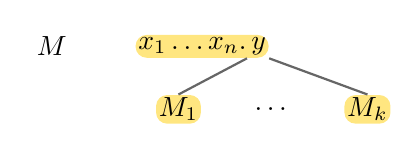
\begin{tikzpicture}
\node 		(BTM) at (-23pt,0)					{$\BT M \eqdef$};
\node[n] 	(y) 	at (1.1,0) 		{$\lam x_1\dots x_n.\,y$};
\node[n] 	(BTM1) 	at (.8,-.8) 	{$\BT{M_1}$};
\node 				at (2,-.8) 		{\dots};
\node[n] 	(BTM2) 	at (3.2,-.8) 	{$\BT{M_k}$};
\draw[b] ($(y.south east)+(-8pt,0)$) -- (BTM1.north);
\draw[b] (y.south east) -- (BTM2.north);
\end{tikzpicture}
\]
\item $\BT{M} \eqdef \bot$, otherwise. The constant $\bot$ represents the absolute lack of information.
\end{enumerate}
\end{definition}
\end{minipage}

\begin{example}\label{ex:BTs} 
Using the terms from Example~\ref{ex:combinators} and \eqref{eq:fpc}, let us construct some Böhm trees.
\bsub
\item If $M$ has a $\beta$-normal form $N$ then, up to isomorphism, $\BT{M} = N$. E.g., $\BT{\comb{DI}} = \comb{I}$.
\item Since $\Om$ and $\comb{YK}$ have no hnf, we get $\BT{\Om} = \BT{\comb{YK}} = \bot$.
\item If $Y$ is an fpc, then $\BT{Y} = \lam f.f(f(f(\cdots)))$. Thus, $\BT{\comb{Y}} = \BT{\Bible} = \BT{\Theta_l}$.
\item\label{ex:BTs4} 
	Using the fpc $\comb{Y}$, one can define \lam-terms $\comb{E}_x,\comb{O}_x$ satisfying
	$\comb{E}_x =_\beta {[}\Om, [\Om x, \comb{E}_x]]$ and 
	$\comb{O}_x =_\beta {[}\Om x, [\Om, \comb{O}_x]]$. 
These two \lam-terms both construct a `stream' $[M_1,[M_2,[M_3,[\cdots]]]]$, but the former places $\Om x$ at even positions and $\Om$ at odd ones, while the latter does the converse.
This difference is however forgotten in their Böhm trees:
\[
	\BT{\comb{E}_x} = \BT{\comb{O}_x} = [\bot,[\bot,[\bot,[\bot,[\,\cdots]]]]]\hfill\textrm{ (inline depiction of a tree)}
\]
\item Check that, given $\comb{R} = \lam ylx.x(y(xl))$, we have $\BT{\comb{YR}l} = \lam x_0.x_0(\lam x_1.x_1(\lam x_2.x_2(\cdots)))$.
\esub
\end{example}

The B\"ohm tree equality induces an equivalence on \lam-terms: $M =_\cB N$ iff $\BT{M} = \BT{N}$. 
As shown in \cite{Levy76,Wadsworth78}, $\cB$ is a \emph{\lam-theory} because it contains $=_\beta$ and is \emph{compatible} with abstraction and application: $M =_\cB M'$ entails $\lam x.M =_\cB \lam x.M'$, $MN =_\cB M'N$ and $NM =_\cB NM'$.

\subsection{The \lamI-calculus}\label{ssec:lamI}

The set $\LamI$ of \lamI-terms is the subset of $\Lam$ consisting of those \lam-terms 
in which every abstraction binds \emph{at least} one occurrence of the abstracted variable.
Note that  $\red[\beta]$ induces a reduction on $\LamI$ since $M\in\LamI$ and $M \red[\beta] N$ entail $N\in\LamI$. 
In other words, the property of being a \lamI-term is preserved by $\red[\beta]$.
Similarly, the \lamI-calculus inherits from \lam-calculus all the notions previously defined like head reduction, Böhm trees, etc.
For convenience, we consider an alternative definition of $\LamI$ simultaneously defining $\lamI$-terms and their sets of free variables.

\begin{definition}\label{def:LamI}\mbox{}
\bsub
\item For all $X \subseteq \Var$, $\LamI(X)$ is defined as 
	the smallest subset of $\Lam$ such that:
\[
	\infer{x\in\LamI(\set{x})}{}\qquad
	\infer{\lam x.M\in\LamI(X\setminus\set{x})}{M\in\LamI(X)\quad x\in X}\qquad
	%\infer{\lam x.M\in\LamI(X)}{M\in\LamI(\set{x}\cup X)\quad x\notin X}\qquad
	\infer{MN\in\LamI(X\cup Y)}{M\in\LamI(X) & N\in\LamI(Y)}
\]
%The above definition differs from the usual definition of (regular) 
%\lam-terms with their set of free variables only in the side condition of 
%the second clause (namely, `$x\in X$').
\item Finally, the set of all \lamI-terms is given by 
	the disjoint union
	$\LamI = \bigdunion_{X\subseteq\Var}\LamI(X)$.
%$\LamI = \set{ M\in\Lam \mid \exists X\subseteq\Var\,.\, M\in\LamI(X)}$.
\esub
\end{definition}

\begin{remark}\label{rem:aboutLambdaI}\mbox{}
\bsub
\item Note that $M \in \LamI(X)$ means that $M$ is a \lamI-term such that $\fv{(M)}=X$.
As a consequence, if $M\in\LamI(X)$ then the set $X$ must be finite.
\item\label{rem:aboutLambdaI2} 
	Each set $\LamI(X)$ is closed under $\beta$-conversion.
\item Our examples $\comb{I},\comb{B},\comb{D},\Om,\comb{Y},\Bible,\Theta_l,\comb{E}_x,\comb{O}_x,\comb{YR}l$ are \lamI-terms, while $\comb{K},\comb{F},\comb{YK}\notin\LamI$.
\esub
\end{remark}

\begin{definition}
A \emph{\lamI-theory} $\cT$ is given by an equivalence $\mathord{=_\cT} \subseteq \LamI^2$ containing $\beta$-conversion and compatible with application and abstraction. 
In the context of \lamI-calculus, 
the compatibility with abstraction becomes: 
$M =_\cT M'$ and $x\in\fv(M)\cap\fv(M')$ 
imply $\lam x.M =_\cT \lam x.M'$.
\end{definition}
The only subtlety in the definition above stands in the side condition on the compatibility with abstraction.
However, this small difference has significant consequences: e.g., the theory axiomatized by equating all terms without a $\beta$-nf is consistent as a \lamI-theory, but inconsistent as a \lam-theory.
The following theorem collects the main properties of the \lamI-calculus.
\begin{theorem}\label{thm:LamIMainProps}\mbox{}
\bsub
\item\label{thm:LamIMainProps1} 
	Every computable numerical function is \lamI-definable~\cite[Thm.~9.2.16]{Bare}.
\item\label{thm:LamIMainProps2} 
	Strong and weak $\beta$-normalization coincide for the \lamI-calculus~\cite[Thm.~11.3.4]{Bare}.
\item\label{thm:LamIMainProps3} 
	Every \lam-theory is also a \lamI-theory, while the converse does not hold. 
\esub
\end{theorem}
%Some comments on these results.
%To prove \eqref{thm:LamIMainProps1} (aka.~Turing completeness) it is sufficient to redefine Church's numeral zero $\comb{c}_0^\comb{I} = \lam xy.x\comb{II}y\in\LamI$ (see ). 
%Consequently, the \lam-terms $\comb{E}_x,\comb{O}_x$ from Example~\ref{ex:BTs}\eqref{ex:BTs4} can be defined in such a way that they belong to $\LamI$.


By \eqref{thm:LamIMainProps3}, Böhm trees induce a \lamI-theory, but we argue that this theory does not respect the spirit of $\LamI$. 
E.g., the variable $l$ is never erased along the reduction of, say, $\Bible$, but it disappears in its B\"ohm tree. Using the terminology of \cite{Bare}, one says that $l$ is \emph{pushed to infinity} in $\BT{\Bible}$.
This shows that the Böhm tree of the \lamI-term $\lam l.\Bible\in\LamI$ is not a $\lamI$-tree: the outer \lam-abstraction `$\lam l$' does not bind any free occurrence of $l$ in $\BT{\Bible} = \lam f.f(f(f(\,\cdots)))$.

% !TEX root = ../CerdaMS.tex

\section{Ohana trees}\label{sec:MemTrees}

% BEGIN unchanged author include/MTrees.tex
% !TEX root = ../CerdaMS.tex

\begin{figure}
	\centering
	\scalebox{.85}{%
	% MT of E_x
	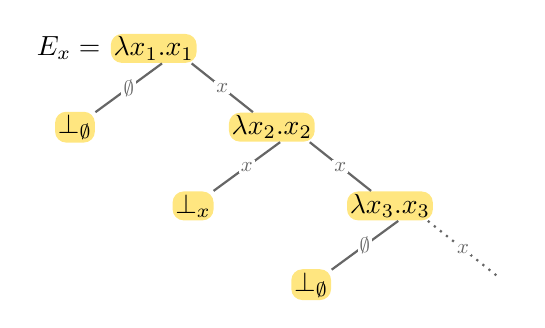
\begin{tikzpicture}[baseline]
		\node[n] 	(E-lx1) 					{$\ensuremath{\lambda}x_1.x_1$};
		\node[left=0pt of E-lx1.west] {$\MT{\comb E_x} =$};
		\node[n] 	(E-bot1) 	at (-1,-1) 		{$\bot_\emptyset$};
		\node[n] 	(E-lx2) 	at (1.5,-1) 		{$\ensuremath{\lambda}x_2.x_2$};
		\node[n] 	(E-bot2) 	at (0.5,-2) 		{$\bot_{\set x}$};
		\node[n] 	(E-lx3) 	at (3,-2) 		{$\ensuremath{\lambda}x_3.x_3$};
		\node[n] 	(E-bot3) 	at (2,-3) 		{$\bot_\emptyset$};
		\node 		(E-inf) 	at (4.5,-3) 		{};
		\draw[b] ($(E-lx1.south)+(3pt,0)$) to[pos=.5] node[m]{$\emptyset$} (E-bot1);
		\draw[b] ($(E-lx1.south east)-(2pt,0)$) to[pos=.5] node[m]{$\set x$} (E-lx2);
		\draw[b] ($(E-lx2.south)+(3pt,0)$) to[pos=.5] node[m]{$\set x$} (E-bot2);
		\draw[b] ($(E-lx2.south east)-(2pt,0)$) to[pos=.5] node[m]{$\set x$} (E-lx3);
		\draw[b] ($(E-lx3.south)+(3pt,0)$) to[pos=.5] node[m]{$\emptyset$} (E-bot3);
		\draw[b,dotted] ($(E-lx3.south east)-(2pt,0)$) to[pos=.5] node[m]{$\set x$} (E-inf);
	\end{tikzpicture}
	% MT of O_x
	\quad
	\begin{tikzpicture}[baseline,overlay]
			\node[n] 	(O-lx1) 					{$\ensuremath{\lambda}x_1.x_1$};
		\node[left=0pt of O-lx1.west] {$\MT{\comb O_x} =$};
		\node[n] 	(O-bot1) 	at (-1,-1) 		{$\bot_{\set x}$};
		\node[n] 	(O-lx2) 	at (1.5,-1) 		{$\ensuremath{\lambda}x_2.x_2$};
		\node[n] 	(O-bot2) 	at (0.5,-2) 		{$\bot_\emptyset$};
		\node[n] 	(O-lx3) 	at (3,-2) 		{$\ensuremath{\lambda}x_3.x_3$};
		\node[n] 	(O-bot3) 	at (2,-3) 		{$\bot_{\set x}$};
		\node 		(O-inf) 	at (4.5,-3) 		{};
		\draw[b] ($(O-lx1.south)+(3pt,0)$) to[pos=.5] node[m]{$\set x$} (O-bot1);
		\draw[b] ($(O-lx1.south east)-(2pt,0)$) to[pos=.5] node[m]{$\set x$} (O-lx2);
		\draw[b] ($(O-lx2.south)+(3pt,0)$) to[pos=.5] node[m]{$\emptyset$} (O-bot2);
		\draw[b] ($(O-lx2.south east)-(2pt,0)$) to[pos=.5] node[m]{$\set x$} (O-lx3);
		\draw[b] ($(O-lx3.south)+(3pt,0)$) to[pos=.5] node[m]{$\set x$} (O-bot3);
		\draw[b,dotted] ($(O-lx3.south east)-(2pt,0)$) to[pos=.5] node[m]{$\set x$} (O-inf);
	\end{tikzpicture} 
	% MT of YRl
	\hspace{5cm}
	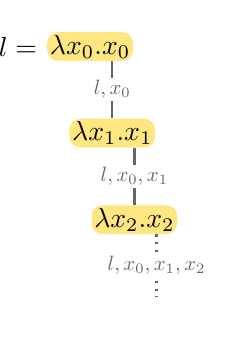
\begin{tikzpicture}[baseline]
		\node[n] 	(YR-l0) 					{$\ensuremath{\lambda}x_0.x_0$};
		\node[left=0pt of YR-l0.west] {\llap{$\MT{\comb Y\comb Rl} =$}};
		\node[n]	(YR-l1)		at (8pt,-1.1)		{$\ensuremath{\lambda}x_1.x_1$};
		\node[n]	(YR-l2)		at (16pt,-2.2)		{$\ensuremath{\lambda}x_2.x_2$};
		\node		(YR-inf)	at (24pt,-3.3)		{};
		\draw[b] ($(YR-l1)+(0,26pt)$) to[pos=.5] node[m]{$\set{l,x_0}$} (YR-l1);
		\draw[b] ($(YR-l2)+(0,26pt)$) to[pos=.5] node[m]{$\set{l,x_0,x_1}$} (YR-l2);
		\draw[b,dotted] ($(YR-inf)+(0,26pt)$) to[pos=.5] 
			node[m]{$\set{l,x_0,x_1,x_2}$} (YR-inf);
	\end{tikzpicture}%
	}
	\caption{Examples of Ohana trees of \lamI-terms.}\label{fig:MTrees}
\end{figure}
% END unchanged author include/MTrees.tex


We have seen that Böhm trees are not well-suited for representing \lamI-terms faithfully, because variables that are never erased along the reduction are forgotten (i.e., pushed into infinity).
We now introduce a notion of evaluation tree that records all variables that are pushed along each path, 
 ensuring that none are forgotten, whether they remain in passive position or not.

\subsection{The coinductive definition}

For every finite set $X\subseteq\Var$, written $X\subf \Var$, we introduce a constant $\bot_X$ representing any looping $M\in\LamI(X)$. 
Intuitively, the \emph{Ohana tree} of a \lamI-term $M$ is obtained from $\BT{M}$ by annotating each subtree (also 
$\bot$) with the free variables of the \lam-term that generated it.

\Needspace{3cm}
\begin{definition}\label{def:memorytrees4LamI}
The \emph{Ohana tree} of a term $M\in\LamI(X)$ is coinductively defined as follows:
\bsub
\item If $M \redd[h] \lam x_1\dots x_n.yM_1\cdots M_k$ with $y\in 
X\cup\set{\vec x}$, $M_i\in\LamI(X_i)$ (for $1\le i \le k$), then\smallskip
\[
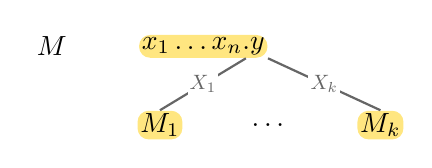
\begin{tikzpicture}
\node 		(MTM) 	at (-22pt,0)				{$\MT M \eqdef$};
\node[n] 	(y) 	at (1.15,0) 		{$\lam x_1\dots x_n.y$};
\node[n] 	(MTM1) 	at (.6,-1) 	{$\MT{M_1}$};
\node 				at (2,-1) 		{\dots};
\node[n] 	(MTM2) 	at (3.4,-1) 	{$\MT{M_k}$};
\draw[b] ($(y.south east)+(-8pt,0)$) to[pos=0.5]node[m]{$X_1$} (MTM1.north);
\draw[b] (y.south east) to[pos=0.5]node[m]{$X_k$} (MTM2.north);
\end{tikzpicture}
\]
\item $\MT{M} \eqdef \bot_X$, otherwise. Recall that $X = \fv(M)$, 
since $M\in\LamI(X)$.
\esub
\end{definition}

We sometimes use an inline presentation of Ohana trees, 
by introducing application symbols annotated with the sets $X_i$, as in 
$\lam x_1\ldots x_n.y\cdot^{X_1}T_1\cdots^{X_k}T_k$.
\begin{example}\label{ex:MTs}\mbox{}
\bsub
\item $\MT{\comb{I}} = \lam x.x$, $\MT{\comb{D}} = \lam x.x\cdot^{\set{x}}x$, $\MT{\comb{B}} = \lam fgx.f\cdot^{\set{g,x}}(g\cdot^{\set{x}}x)$.
\item $\MT{\Om} = \MT{\lam y.\Om y} = \bot_{\emptyset}$, $\MT{\Om x} = \bot_{\set x}$. More generally: $\MT{\Om \vec x} = \bot_{\set{x_1,\dots,x_n}}$. 
\item  $\MT{\comb{Y}} = \lam f.f\cdot^{\set{f}}(f\cdot^{\set{f}}(f\cdot^{\set{f}}(\,\cdots)))$. 
	In fact, it is easy to check that for all \emph{closed} fpcs $Y\in\LamI$, we have $\MT{Y} = \MT{\comb{Y}} \cong \BT{\comb{Y}}$.
\item In $\MT{\Bible}$ the variable $l$ which is pushed into infinity becomes visible: $\MT{\Bible} =\MT{\Theta_l} = \lam f.f\cdot^{\set{f,l}}(f\cdot^{\set{f,l}}(f\cdot^{\set{f,l}}(\,\cdots)))$. Thus $\MT{\Bible} \neq \MT{\Theta_x}$ when $x\neq l$.
\esub
\end{example}

Other examples of Ohana trees are depicted in Figure~\ref{fig:MTrees}.
Note that the Ohana trees of $\comb{E}_x$ and $\comb{O}_x$ are now distinguished.
The interest of ${\comb{YR}l}$ is that it pushes into infinity an increasing amount of variables: 
\[\comb{YR}l =_\beta \lam x_0.x_0((\comb{YR})(x_0l)) =_\beta \lam x_0.x_0(\lam x_1.x_1((\comb{YR})(x_1(x_0l))))\, {=_\beta} \cdots\]
So---at the limit---infinitely many variables are pushed into infinity (but only $l$ is free).

\begin{remark} If $M\in\LamI$ has a $\beta$-nf $N$, then there is an isomorphism $\MT{M}\cong N$.
In fact, since $N$ is finite, it is possible to reconstruct all the labels in $\MT{M}$.  
%Formally, proceed by induction on the structure of $\MT{M}$ for $(\Rightarrow)$, and of $N$ for $(\Leftarrow)$.
\end{remark}

We are going to show that Ohana trees are invariant under $\beta$-reduction (Prop.~\ref{prop:InvariantUnderBeta} plus Thm.~\ref{thm:MTbijApp}), and that the equality induced on \lamI-terms is a \lamI-theory (Corollary~\ref{cor:MisALamITheory}).

\subsection{The associated approximation theory}

We introduce a theory of program approximation that captures Ohana trees, by adapting the well-established approach originally developed for Böhm trees~\cite{Levy76,Wadsworth78} (see also \cite[Ch.~14]{Bare}).
We start by defining the approximants with memory, corresponding to finite Ohana trees.

\begin{definition}\label{def:approximants}\mbox{}
\bsub
\item \label{def:approximants1}
	The set of \emph{approximants with memory} is 
	$\Appset \eqdef \bigdunion_{X\subf \Var} \Appset(X)$, 
	where $\Appset(X)$ is defined by (for $A_i\in\Appset(X_i)$, $X_i\subseteq X$, 
	$y\in X\cup\set{\vec x}$ and $\vec x\in\bigcup_{i=1}^k X_i$):
	\bnf[\Appset(X)]{A}{ \bot_X \mid \lam x_1\ldots x_n.yA_1\cdots A_k}
	
%\item We extend $\fv(\cdot)$ to $\Appset$ by adding $\fv(\bot_X) = X$, thus $\fv(A) = X$ stands for $A\in\Appset(X)$.
\item We define $\mathord{\MTle} \subseteq \Appset^2$ as 
the least partial order closed under the following rules:
\[
	\infer{\bot_X\MTle A}{A\in\Appset(X)}\qquad
	\infer{\lam x_1\dots x_n.y\, A_1\cdots A_k \MTle \lam x_1\dots x_n.y\, A'_1\cdots A'_k}{A_i\MTle A'_i&A_i,A'_i\in\Appset(X_i)&\textrm{for all }1\le i \le k&\vec x\in\set{y}\cup\big(\bigcup_{i=1}^k X_i\big)}
\]
\esub
\end{definition}

Each $(\Appset(X), \MTle)$ is a pointed poset (partially ordered set) with bottom element $\bot_X$, while the poset $(\Appset,\MTle)$ is not pointed because it has countably many minimal elements.
Note that we do not annotate the application symbols 
in $A\in\Appset$ with the sets of variables $X_i$, 
since the labels in its $\bot$-nodes carry enough information 
to reconstruct the finite Ohana tree associated with $A$.
%Contrarily to the case of memory tree, we do not annotate the application symbol in $A\in\LamI$, since the labels in its $\bot$-nodes carry enough information to reconstruct the finite memory tree associated with $A$.
%Remark that $(\Appset,\MTle)$ is not \emph{pointed} as a poset (partially ordered set), because it has countably many minimal elements $\bot_X$. 
%However, each $\Appset(X)$ has  its bottom element $\bot_X$.
%Also, we do not need to annotate the application symbol in $A\in\LamI$, 
%since the labels in its $\bot$-nodes carry enough information to 
%reconstruct 
%the finite memory tree associated with $A$.

\newcounter{lem:bijAppsetfinmemtrees}
\setcounter{lem:bijAppsetfinmemtrees}{\thetheorem}
\begin{lemma}
\label{lem:bijAppset_finmemtrees}\label{lem:bijAppsetfinmemtrees}
There is a bijection between $\Appset$ and the set of finite Ohana trees of \lamI-terms.
\end{lemma}

We now give the recipe to compute the set of approximants with memory of a \lamI-term.

\begin{definition}\mbox{}
\bsub
\item The \emph{direct approximant} of $M\in\LamI(X)$ is given by:
\[
	\dirapp{M} \eqdef 
	\begin{cases}
	 \lam x_1\ldots x_n.y\,\dirapp{M_1}\cdots \dirapp{M_k},&\textrm{if }M = \lam x_1\ldots x_n.yM_1\cdots M_k,\\	
	\bot_X,&\textrm{otherwise.}
	\end{cases}
\]
\item The set $\Appof{M}$ of \emph{approximants with memory of $M\in\LamI$} is defined by:
\[
	\Appof{M} \eqdef \set{ A\in\Appset \mid \exists N\in\LamI\,.\, M\redd[\beta]N \textrm{ and }A\MTle \dirapp{N}}
\]
\esub
\end{definition}

\begin{remark} \label{rem:appof-M-fv-M}
	For all $M \in \LamI(X)$, we have $\dirapp M \in \Appset(X)$ and $\Appof M \subseteq \Appset(X)$.
\end{remark}

\begin{example}\mbox{}
\bsub
\item $\Appof{\comb{D}} = \set{\bot_\emptyset, \lam x.x\bot_{\set x}, 
		\comb{D}}$, 
	$\Appof{\Om} = \set{\bot_{\emptyset}}$%
%	, $\Appof{\Om x} = \set{\bot_{\set{x}}}$%
	.
\item $\Appof{\comb{Y}} = \set{\bot_\emptyset} \cup 
		\set{ \lam f.f^n(\bot_{\set f}) \mid n\in\Nat} $.
\item $\Appof{\Bible} = \set{\bot_{\set{l}}} \cup 
		\set{ \lam f.f^n(\bot_{\set{f,l}}) \mid n\in\Nat} $.
\item $\Appof{\comb{YR}l} = \set{\bot_{\set{l}},
	\lam x_0.x_0(\bot_{\set{x_0,l}}),
	\lam x_0.x_0(\lam x_1.x_1(\bot_{\set{x_0,x_1,l}})), \dots}$.
\esub
\end{example}

\newcounter{lem:DirApp}
\setcounter{lem:DirApp}{\thetheorem}
\begin{lemma}\label{lem:DirApp}\mbox{}
\bsub
\item\label{lem:DirApp1} 
	For every $M,N\in\LamI$, $M\bred N$ entails  $\dirapp{M} \MTle \dirapp{N}$.
\item\label{lem:DirApp2} 
	For all $M\in\LamI(X)$, $\Appof{M}$ is an ideal of the poset $(\Appset(X),\sqsubseteq)$. More precisely:
	\begin{enumerate}
	\item
		non-emptiness: $\bot_X\in \Appof{M}$;
	\item
		downward closure: $A\in \Appof{M}$ and $A'\MTle A$ imply $A'\in\Appof{M}$;
	\item
		directedness: $\forall A_1,A_2\in\Appof{M},\exists A_3\in\Appof{M}$ such that $A_1\MTle A_3 \sqsupseteq A_2$.
	\end{enumerate}
\esub
\end{lemma}
\begin{proof}
\bsub
\item
By an easy induction on the structure of $M\in\LamI(X)$, using Remarks~\ref{rem:hnfs} and \ref{rem:aboutLambdaI}.
\item (a) and (b) are trivial. 
	For (c), define $\MTlub$ by setting: 
	$\bot_X\MTlub A = A\MTlub \bot_X= A$, $x\MTlub x = x$, 
	if $A_1,A'_1$ and $A_2, A'_2$ are compatible, 
	then $(\lam x.A_1)\MTlub (\lam x.A'_1) = \lam x.(A_1\MTlub A'_1)$ 
	and $A_1A_2\MTlub A'_1A'_2 = (A_1\MTlub A'_1) (A_2\MTlub A'_2)$. 
	Check that $A_3 = A_1 \MTlub A_2$ is their supremum.
\qedhere
\esub
\end{proof}

The next result shows that $\beta$-convertible terms share the same the set of approximants.\par\addvspace{1.5ex}

\noindent\begin{minipage}{\textwidth}
\newcounter{prop:InvariantUnderBeta}
\setcounter{prop:InvariantUnderBeta}{\thetheorem}
\begin{proposition}\label{prop:InvariantUnderBeta}
	Let $M,N\in\LamI(X)$. If $M\red[\beta] N$, then $\Appof{M} = \Appof{N}$.
\end{proposition}

\begin{proof}By confluence of $\red[\beta]$, using Lemma~\ref{lem:DirApp}\eqref{lem:DirApp1}.
\end{proof}
\end{minipage}

\newcounter{thm:MTbijApp}
\setcounter{thm:MTbijApp}{\thetheorem}
\begin{theorem}\label{thm:MTbijApp} 
%For all $M\in\LamI$, there is an isomorphism $\MT{M} \cong \Appof{M}$.
	There is a bijection $\mtapp{\cdot}$ between the set of Ohana trees and the set of approximants of \lamI-terms satisfying $\mtapp{\MT{M}} = \Appof{M}$, for all $M\in\LamI$.

\end{theorem}

\begin{proof} From $\MT{M}$ to $\Appof{M}$.
Let $\MT{M}^\star$ be the set of all finite subtrees of $\MT{M}$, 
where each truncated subtree $T$ is replaced by $\bot_{\fv(T)}$.
By Lemma~\ref{lem:bijAppset_finmemtrees}, $\MT{M}^\star\cong\Appof{M}$.

From $\Appof{M}$ to $\MT{M}$. For every finite path $\sigma$ in $\MT{M}$, there is an $A\in\Appof{M}$ representing $\MT{M}$ along $\sigma$. Conclude since $\MT{M}$ is the supremum of all such $\sigma$.
\end{proof}



% !TEX root = ../CerdaMS.tex

\section{A resource calculus with memory}
\label{sec:resource}

%\comrci{With memory or with memories?}

In this section we introduce the \emph{\lamI-resource calculus} refining the (finite) resource calculus~\cite{EhrhardR03}, best known as the target language of Ehrhard and Regnier's Taylor expansion~\cite{Ehrhard.Reg.08}. 
So, the resource calculus is not meant to be a stand-alone language, but rather another theory of approximations for the \lam-calculus.
Before going further, we recall its main properties.

%\subsection{An introduction to resource calculi}

We consider here the promotion-free fragment of the resource calculus introduced in \cite{PaganiT09}.
Its syntax is similar to the \lam-calculus, except for the applications that are of shape $\rt{s}\rb t$, where $\rb t = [\rt{t}_1,\dots,\rt{t}_n]$ is a multiset of resources called \emph{bag}.
The resources populating $\rb t$ are linear as they cannot be erased or copied by $\rt s$, they must be used \emph{exactly once} along the reduction. 
When contracting a term of the form $s = (\lam x.\rt{s'})[\rt{t}_1,\dots,\rt{t}_n]$ there are two possibilities.
\begin{enumerate}
\item If the number of occurrences of $x$ in $\rt{s'}$ is exactly $n$, then each occurrence is substituted by a different $\rt{t}_i$. 
Since the elements in the bag are unordered, there is no canonical bijection between the resources and the occurrences of $x$. 
The solution consists in collecting all possibilities in a formal sum of terms, the sum representing an inner-choice operator.
\item If there is a mismatch between the number of occurrences and the amount of resources, then $s$ reduces to the empty-sum, $\esum{}$. From a programming-language perspective, this can be thought of as a program terminating abruptly after throwing an uncaught exception.
\end{enumerate}
The first-class citizens of the resource calculus are therefore \emph{finite sums} of resource terms, that are needed to ensure the (strong) confluence of reductions. Another important property is strong normalization, that follows from the fact that no resource can be duplicated.

\subsection{\lamI-resource expressions and \lamI-resource sums}

Our version of the resource calculus is extended with labels representing the memory of free variables that were present in the \lamI-term they approximate.
Just like in \cref{def:approximants}\eqref{def:approximants1} 
we endowed the constant $\bot$ with a finite set $X$ of variables, 
here we annotate:
\begin{itemize}
\item the empty bag $1$ of resource terms, since an empty bag of approximants of $M$ should remember the free variables of $M$;
\item the empty sum $\esum{}$ of resource terms. Indeed, if a resource term vanishes during reduction because of the mismatch described above, its free variables should be remembered.
\end{itemize}
%We now rigorously define the terms of our modified resource calculus, 
%as well as the bags used as arguments of applications.
%Then, we extend this syntax to finite sums of terms, 
%on which the dynamics of the calculus is acting.

\begin{definition} \label{def:rterms}\mbox{}
\bsub\item
	For all $X \subf \Var$, the sets $\rterms(X)$ and $\rterms*(X)$
	are defined by induction:
	\begin{gather*}
		\infer{ x \in \rterms(\set{x}) }{} \qquad
		\infer{ \lam x.\rt{s} \in \rterms(X \setminus \set{x}) }
			{ \rt{s} \in \rterms(X) & x \in X } \qquad
		\infer{ \rt{s}\rb{t} \in \rterms(X \cup Y) }
			{ \rt{s} \in \rterms(X) & \rb{t} \in \rterms*(Y) } \\
		\infer{ 1_X \in \rterms*(X) }{} \qquad
		\infer{ [\rt{t}_0,\dots,\rt{t}_n] \in \rterms*(X)}
			{ \rt{t}_0 \in \rterms(X) & \cdots & \rt{t}_n \in \rterms(X) }
	\end{gather*}
\item
	The set $\rterms$ of \emph{\lamI-resource terms} and
	the set $\rterms*$ of \emph{bags} are given by:
	\[	\rterms \eqdef \bigdunion_{X \subf \Var} \rterms(X)
		\quad \text{and}\quad
		\rterms* \eqdef \bigdunion_{X \subf \Var} \rterms*(X). \]
\esub
\end{definition}
As a matter of notation, we let $\rterms**$ denote either $\rterms$ or $\rterms*$, indistinctly but coherently.
We call \emph{resource expressions} generic elements $s,t\in\rterms**$. 
We denote the union of two bags $\rb{t}, \rb{u}\in\rterms*(X)$ multiplicatively by $\rb{t} \cdot \rb{u}$,
whose neutral element is the empty bag, $1_X$.
%whence the empty bag $1_X$ is the neutral element.

\Needspace{2cm}
\begin{remark}\label{rem:aboutresourceterms}\mbox{}
\bsub
\item
In every \lamI-resource term of the form $\lam x.s$, the variable $x$ must occur freely in $s$: it may appear in the undecorated underlying term, or in the \enquote{memory} $X$ decorating $1_X$.
Therefore, it makes sense to define $\fv(\rt s) \eqdef X$ whenever $\rt{s} \in \rterms**(X)$.
\item\label{rem:aboutresourceterms2}
Each set $\rterms*(X)$ is isomorphic to the monoid of
multisets of elements of $\rterms(X)$.
Notice that $\rterms*$ is \emph{not} the set of all bags
of elements of $\rterms$, just its subset of bags
whose elements \emph{have the same free variables}
(and so inductively in the subterms).
\esub
\end{remark}

\begin{example}\label{ex:resourceterms}\mbox{}
\bsub
\item The identity $\comb{I}$ belongs to $\rterms$, whereas the projections do not: $\comb{K},\comb{F}\notin\rterms$.
\item Note that $\lam xy.x1_{\emptyset}\notin\rterms$ since $y\notin\fv(x1_{\emptyset})$, but $\lam xy.x1_{\set{y}}\in\rterms$ because $y\in\set{y}$.
\item The terms $\comb{D}_0 = \lam x.x1_{\set{x}}$ and $\comb{D}_{n+1} = \lam x.x[x,\ldots,x]$, where the bag contains $n+1$ occurrences of $x$, are \lamI-resource terms. By Remark~\ref{rem:aboutresourceterms}\eqref{rem:aboutresourceterms2}, we obtain:
\item $[x,y] \notin \rterms*$, while $[x, x[x], x[\lam y.y,\lam y.y[y]], (\lam y.y)[x],  \lam y.y1_{\set x}] \in \rterms*(\set{x})\subseteq\rterms*$.
\esub
\end{example}

We consider resource expressions up to $\alpha$-equivalence, under the proviso that abstractions bind linear occurrences of variables as well as occurrences in the memory of empty bags. For instance, $\lam xyz.x1_{\set{x}}1_{\set{x,y,z}}$ and  $\lam x'y'z.x'1_{\set{x'}}1_{\set{x',y',z}}$ are considered $\alpha$-equivalent. 

\begin{definition}\label{def:frsums}
	For all $X \subf \Var$, the set $\frsums[X]**$
	of \emph{sums of \lamI-resource terms} (\enquote{\mbox{resource sums}}, for short)
	is defined as the $\Nat$-semimodule
	of finitely supported formal sums of expressions in $\rterms**(X)$,
	with coefficients in $\Nat$.
	Explicitly, it can be presented as:
	\bnf[ \frsums[X]** ]{ \rs{s},\rs{t} }
		{ \esum X \mid \rt r\mid \rt{r} + \rs{s} }
		[ \text{for $\rt{r} \in \rterms**(X)$} ]
	quotiented by associativity and commutativity of $+$,
	as well as neutrality of $\esum X$.
\end{definition}

Note that $\rterms**(X)\subseteq\frsums[X]**$, that is, resource expressions are assimilated to the corresponding
one-element sum.
The constructors of the calculus are extended
to resource sums by (bi)linearity, \emph{i.e.}
for $\rt{s} \in \rterms(X)$, $\rs{s} \in \frsums[X]$, 
$\rb{t} \in \rterms*(Y)$, $\rbs{t} \in \frsums[Y]*$,
$\rt{u} \in \rterms(Y)$ and $\rs{u} \in \frsums[Y]$, we have:
\[
	\begin{array}{llll}
	(\rt{s}+\rs{s}) \rb{t} \eqdef \rt{s}\rb{t} + \rs{s}\rb{t},&
	\esum X \rb{t} \eqdef \esum {X \cup Y},&
	\lam x.(\rt{s}+\rs{s}) \eqdef \lam x.\rt{s} + \lam x.\rs{s},&
	\lam x.\esum X \eqdef \esum {X \setminus \set{x}},\\[1ex]
	\rt{s} (\rb{t}+\rbs{t}) \eqdef \rt{s}\rb{t} + \rt{s}\rbs{t},&
	\rt{s}\esum Y \eqdef \esum {X \cup Y},&
	[\rt{u} + \rs{u}] \cdot \rb{t} \eqdef [\rt{u}]\cdot\rb{t}
		+ [\rs{u}]\cdot\rb{t},&	
	[\esum Y] \cdot \rb{t} \eqdef \esum Y.
	\end{array}
\]
Therefore, if $\esum X$ occurs in $s$ not as a summand but as a proper subterm, then $s = \esum{\fv(s)}$.

\subsection{Memory substitution and resource substitution}

While the usual finite resource calculus is completely linear, the variables we store in the memory of $1_X$ and $\esum X$ are not. 
The memory $X$ remembers the variables present in $X$ not their amounts, this is the reason why it is modelled as a set, not as a multiset. 
This consideration leads us to define two kinds of substitutions.

The (non-linear) \emph{memory substitution} of a set $Y\subf\Var$ for a variable $x$ in a \lamI-resource term $s$ does not interact with the linear occurrences of $x$ in $s$ (\emph{i.e.}, they remain unchanged), it just replaces the \enquote{memory} of $x$ in the empty bags with the content of $Y$.

\begin{definition} \label{def:msubst}\mbox{}
\bsub
\item For all $X,Y \subf \Var$ and $x \in \Var$, define
	\[
	X \msubst Y \eqdef \begin{cases}
		X \setminus \{x\} \cup Y, 
			& \text{if $x \in X$,} \\
		X, & \text{otherwise.}\\
	\end{cases}
	\]
	\item Given $\rt{s} \in \rterms**(X)$, the \emph{memory substitution} of  $x$ by $Y\subf\Var$ in $\rt{s}$ is the resource term $\rt{s} \msubst Y$ defined as follows (for $x \neq y$ and, in the abstraction case, $y \notin Y$):
	\begin{flalign*}
		x \msubst Y & \eqdef x, &
		1_X \msubst Y & \eqdef 1_{X\msubst Y},&
		(\rt{s}\rb{t}) \msubst Y & \eqdef 
			(\rt{s}\msubst Y)(\rb{t}\msubst Y),  \\
		y  \msubst Y & \eqdef y,  &
		(\lam y.\rt{s}) \msubst Y & \eqdef \lam y.\rt{s} \msubst Y,	&
		([\rt s] \cdot \rb t) \msubst Y & \eqdef
			[\rt s \msubst Y] \cdot (\rb t \msubst Y).
	\end{flalign*}
\esub			
\end{definition}

We now define the \emph{resource substitution} of a bag $\rb u$ for $x$ in $\rt s$, whose effect is twofold.
1)~It non-deterministically replaces each linear occurrence of $x$ with a 
resource from the bag (as usual).
2) It applies the memory substitution of $x$ by $\fv(\rb u)$ to the resulting sum of terms.

\begin{definition} \label{def:rsubst}
	Given $\rt s \in \rterms**(X)$, $x \in \Var$ and $\rb u \in \rterms*(Y)$,
	the \emph{resource substitution} of $x$ by $\rb u$ in $\rt s$
	is the resource sum $\rt s \rsubst u \in \frsums[X \msubst Y]**$
	defined as follows:
	\begin{align*}
		x \rsubst u & \eqdef 
			\begin{cases}
			\rt u,& \text{if $\rb u = [\rt u]$},\\
			\esum Y, & \text{otherwise},
			\end{cases} &
		(\rt{s}\rb{t}) \rsubst u & \eqdef 
			\sum_{\rb u = \rb v \cdot \rb w}
			(\rt{s}\rsubst v)( \rb{t}\rsubst w),\\
		y  \rsubst u & \eqdef 
			\begin{cases}
			y, & \text{if $\rb u = 1_Y$,} \\
			\esum {\set y}, & \text{otherwise},
			\end{cases}&
		1_X \rsubst u & \eqdef 
			\begin{cases}
			1_{X \msubst Y}, & \text{if $\rb u = 1_Y$}, \\
			\esum {X \msubst Y}, & \text{otherwise,} \\
			\end{cases}\\
		(\lam y.\rt{s}) \rsubst u & \eqdef 
			\lam y.\rt{s} \rsubst u, &
		([\rt s] \cdot \rb t) \rsubst u & \eqdef
			\sum_{\rb u = \rb v \cdot \rb w}
			[\rt s \rsubst v] \cdot (\rb t \rsubst w).
	\end{align*}
	with $x \neq y$ and in the abstraction case $y \notin Y$.
	We extend it to sums in $\frsums[X]**$ by setting:
	\begin{align*}
		\esum X \rsubst u & \eqdef \esum {X\msubst Y} &
		(\rt{s} + \rs{s}) \rsubst u & \eqdef 
			\rt{s} \rsubst u + \rs{s} \rsubst u \\
		\rt s \rsubst* {\esum Y} & \eqdef \esum {X \msubst Y} &
		\rt s \rsubst* {(\rb u + \rbs u)} & \eqdef
			\rt s \rsubst u + \rt s \rsubst* {\rbs u}.
	\end{align*}
\end{definition}

It is easy to verify that the definition above does indeed define a resource sum in $\frsums[X \msubst Y]**$, and that it is stable under the quotients of Definition~\ref{def:frsums}.

\begin{definition}The \emph{linear degree} $\deg_x(\rt s)$ of $x \in \Var$
	in some $\rt s \in \rterms**$ is defined by:
	\begin{align*}
	\deg_x(x) & \coloneqq 1, &
	\deg_x(\lam y.\rt s) & \coloneqq \deg_x(\rt s)
		\text{, wlog. $x\neq y$,} &
	\deg_x(1_X) & \coloneqq 0, \\
	\deg_x(y) & \coloneqq 0 ,&
	\deg_x(\rt s \rb t) & \coloneqq \deg_x(\rt s) + \deg_x(\rb t), &
	\deg_x([\rt s] \cdot \rb t) & \coloneqq \deg_x(\rt s) + \deg_x(\rb t).
	\end{align*}

\end{definition}

The next lemma is not strictly needed, but helps understanding resource substitution.

\begin{lemma}\label{lem:aboutressubst}
	Consider $\rt s \in \rterms**(X)$, $x \in \Var$ and
	$\rb u \in \rterms*(Y)$,
	and write $n \coloneqq \deg_x(\rt s)$. Then
	\[	\rt s \rsubst u = 
		\begin{cases}
		\sum\limits_{\sigma \in \mathfrak{S}(n)}
			\rt s\left[ \rt u_{\sigma(1)}/x^{(1)}, \dots, 
			\rt u_{\sigma(n)}/x^{(n)} \right] \msubst Y,
			& \text{if the cardinality of $\rb u$ is $n$,} \\
		\esum {X \msubst Y}, & \text{otherwise,}\\
		\end{cases} 
	\]
	where: $\mathfrak{S}(n)$ is the set of permutations of $\set{1,\dots,n}$;
	$\rt u_1,\dots,\rt u_n$ is any enumeration of the elements in $\rb u$;
	$x^{(1)},\dots,x^{(n)}$ enumerate the occurrences of $x$ in $\rt s$; and
	$\rt s\left[ \rt u_{\sigma(1)}/x^{(1)}, \dots, \rt u_{\sigma(n)}/x^{(n)} \right]$
	is the \lamI-resource term obtained by substituting each element $\rt u_{\sigma(i)}$ for the occurrence $x^{(i)}$.
\end{lemma}
	
	\begin{proof}
	Straightforward induction on $\rt s$.
	\end{proof}

The next Substitution Lemma concerns the commutation of resource substitutions, and is the analogous of \cite[Lemma~2.1.16]{Bare}.
Notice that the assumptions on the substituted variables
are stronger than in the usual resource calculus
\cite[Lemma~2]{Ehrhard.Reg.08},
where only $x \notin Y$ is required.

\newcounter{lem:resource-substitution}
\setcounter{lem:resource-substitution}{\thetheorem}
\begin{lemma}
\label{lem:resource-substitution}
	Given $\rt s \in \rterms**(X)$,
	$\rb u \in \rterms*(Y)$,
	$\rb v \in \rterms*(Z)$,
	and
	$x \in X \setminus Z$, $y \in X \cup Y$,
	\[	\rt s \rsubst u \rsubst v [y] =
		\sum_{\rb v = \rb v' \cdot \rb v''} \rt s \rsubst* {\rb v'} [y]
		\rsubst*{ \rb u \rsubst* {\rb v''}[y] }. \]
\end{lemma}
\begin{proof} By structural induction on $s$, using Lemma~\ref{lem:aboutressubst} in order to apply the induction hypothesis only to those subterms where the hypotheses are actually satisfied.
\end{proof}

\subsection{The operational semantics}

We finally endow resource expressions and resource sums with a notion of reduction $\rred$.

\begin{definition} \label{def:rred}\mbox{}
\bsub
\item
	For each $X \subf \Var$, define the \emph{resource reduction} as a relation between \lamI-resource terms and resource sums, i.e.\
	$\mathord{\rred} \subseteq \rterms**(X) \times \frsums[X]**$:\\[1ex]
	$\infer{ (\lam x.\rt s)\rb t \rred \rt s \rsubst t }{} \qquad
		\infer{ \lam x.\rt s \rred \lam x.\rs s' }{ \rt s \rred \rs s' } \qquad
		\infer{ \rt s \rb t \rred \rs s' \rb t }{ \rt s \rred \rs s' } \qquad
		\infer{ \rt s \rb t \rred \rt s \rbs t' }
			{ \rb t \rred \rbs t' } \qquad
%		\infer{ \rt s \cdot \rb t \rred \rs s' \cdot \rb t }
		\infer{ [\rt s] \cdot \rb t \rred {[\rs s']} \cdot \rb t }
			{ \rt s \rred \rs s' } $\smallskip
\item\label{def:rred3} We extend the reduction relation $\rred$ to resource sums $\frsums[X]** \times \frsums[X]**$, and simultaneously introduce its reflexive closure $\rredr$, as follows: 
%by saying that $\rt s \rred \rs s' $ and $ \rs t \rredr \rs t'$ entail $\rt s + \rs t \rred \rs s' + \rs t'$.
\[
	\infer{\rt s + \rs t \rred \rs s' + \rs t' }{
		\rt s \rred \rs s'
		&
		\rs t \rredr \rs t'
		}
	\qquad
	\infer{\rs t \rredr \rs t'}{\rs t \rred \rs t'}	
	\qquad
	\infer{\rs t \rredr \rs t}{}
\]
%\item
%	We denote by $\rredr$ the reflexive closure of $\rred$. % and by $\redd[\resource]$ its reflexive-transitive closure. 
%\item\label{def:rred3}
%	We extend the reduction relation $\rred$ to resource sums $\frsums[X]** \times \frsums[X]**$ by saying that $\rt s \rred \rs s' $ and $ \rs t \rredr \rs t'$ entail $\rt s + \rs t \rred \rs s' + \rs t'$.
\item
	We denote by $\redd[\resource]$ the reflexive and transitive closure of the relation $\rred$ given in \eqref{def:rred3}. 
\esub
\end{definition}

Observe that $\rred$ is well-defined because $\fv((\lam x.\rt s)\rb t) = \fv(\rt s \rsubst t)$.
Indeed $\fv((\lam x.\rt s)\rb t) = 
\fv(\rt s) \setminus \set x \cup \fv(\rb t)$
with $x \in \fv(\rt s)$, whence $\fv(\rt s \rsubst t) = \fv(\rt s) \msubst {\fv(\rb t)}
= \fv(\rt s) \setminus \set x \cup \fv(\rb t)$.

\begin{example} We use the resource \lamI-terms $\comb{I}$ and $\comb{D}_n$ from Example~\ref{ex:resourceterms}.
\bsub
\item $\comb{D}_0[z]\rred (x1_{\set{x}})\langle[z]/x\rangle = 
	(x\langle[z]/x\rangle)(1_{\set{z}}) + (x\langle1_{\set{z}}/x\rangle)(1_{\set x}\langle [z]/x\rangle) = z1_{\set z}+\esum{\set{z}} = z1_{\set z}$. 
	Similarly, $\comb{D}_0[\comb{I}] \rred \comb{I}1_{\emptyset} 
	\red \esum{\emptyset}$.
%	, while $\comb{D}_1[\comb{I},\comb{I}]\rred \comb{I}[\comb{I}] 
%	\rred \comb{I}$ is a non-zero reduction. 
\item $(\lam x.\comb{D_0}[x])[z]$ has two redexes. Contracting the outermost first gives $(\lam x.\comb{D_0}[x])[z]\rred \comb{D_0}[z]\rred z1_{\set z}$.
Contracting the innermost $(\lam x.\comb{D_0}[x])[z]\rred (\lam x.x1_{\set x})[z]\rred z1_{\set z}$.
\item $\comb{D}_1[\comb{I},\comb{I}]\rred \comb{I}[\comb{I}] + \comb{I}[\comb{I}]\rred \comb{I}+ \comb{I}[\comb{I}]\rred \comb{I}+\comb{I} = 2.\comb{I}$. 
Thus, sums can arise from single terms.
\esub
\end{example}

We show that $\rred$ enjoys the properties of strong confluence and strong normalisation.

\newcounter{the:rred-norm-confl:confl}
\setcounter{the:rred-norm-confl:confl}{\thetheorem}
\begin{theorem} \label{the:rred-norm-confl}\mbox{}
\bsub
\item The reduction $\rred$ is strongly normalising.
	\label{the:rred-norm-confl:norm}
\item $\rred$ is strongly confluent in the following sense:
	for all $\rs s, \rs t_1, \rs t_2 \in \frsums[X]**$
	such that $\rs s \rred \rs t_1$ and $\rs s \rred \rs t_2$,
	there exists $\rs u \in \frsums[X]**$ such that
	$\rs t_1 \rredr \rs u$ and $\rs t_2 \rredr \rs u$.
	\label{the:rred-norm-confl:confl}
\esub 
\end{theorem}

	\begin{proof}\mbox{}
	\bsub
	\item 
	The size $\size s\in\Nat$ of a resource expression $s\in\rterms**$ 
	is defined by structural induction as usual, 
	with base cases $\size{x} = 1$ and $\size{1_X} = 0$, 
	so that $\size{1_X\cdot \rb t} = \size{\rb t}$.
	The \emph{sum-size} of a resource sum $\rs s$ is 
	the finite multiset defined by $\sumsize{\esum{X}} = []$ and 
	$\sumsize{s+\rs t} = [\size{s}]\cdot \sumsize{\rs t}$.
	Sum-sizes are well-ordered by the usual well-founded ordering 
	$\msetlt$ on finite multisets over $\Nat$ 
	(see \cite[\S A.6]{Terese}).
	
	Now, assume that $\rs s \rred\rs s'$. 
	Since the contraction of a redex suppresses an abstraction 
	and there is no duplication, 
	we get $\sumsize{\rs s}\msetlt \sumsize{\rs s'}$. 
	Conclude since $\msetlt$ is well-founded.
	\item The sequence of lemmas leading to the result follows
	a well-trodden path in the resource calculus \cite{Vaux.19,Cerda.24}.
	It is sufficient to check that they generalize to our setting.
%	We give some details in the appendix.
	\qedhere\esub
	\end{proof}

By \eqref{the:rred-norm-confl:confl} above every $\rs s \in \frsums[X]**$ has a unique $\mathrm{r}$-normal form which is denoted $\nf(\rs s)$. 
%We use the notation $t\in\nf(\rs s)$ to express the fact that $\nf(\rs s) = t + \rs s'$, for some $\rs s'$.



% !TEX root = ../CerdaMS.tex

\section{Taylor approximation for Ohana trees}\label{sec:TE4MTs}

In its original formulation, Ehrhard and Regnier's Taylor expansion translates a \lam-term as a power series of iterated derivatives~\cite{Ehrhard.Reg.06}.
We now introduce a \emph{qualitative} Taylor expansion~\cite{ManzonettoP11} specifically designed for the \lamI-calculus, having as target the \lamI-resource calculus.

\subsection{The Taylor approximation}

Intuitively, a qualitative Taylor expansion should associate each term $M \in \LamI(X)$ with a \emph{set} of resource approximants $\TE M \subseteq \rterms(X)$.
Therefore the codomain of $\TE -$ should be $\bigdunion_{X \subf \Var} \parts{\rterms(X)}$, and what we actually define is $\TE M \eqdef (X, \TE* M)$ with $\TE* M \subseteq \rterms(X)$.
Notice that, whereas all previous constructions of disjoint unions
$\bigdunion_{X \subf \Var}$ were formed from genuinely disjoint sets,
this is no longer the case here, as $\emptyset \in \parts{\rterms(X)}$, for all $X$.
\begin{notation}\mbox{}
\bsub
\item For $X \subf \Var$ and $\cX \in \parts{\rterms(X)}$,
	we write $\fv(X,\cX) \eqdef X$.
\item We let $\mathord{\TElt}$ denote the order relation
	on $\bigdunion_{X \subf \Var} \parts{\rterms(X)}$
	such that $(X,\cX) \TElt (Y,\cY)$
	whenever $X = Y$ and $\cX \subseteq \cY$.
	We write $\TElub$ for the corresponding least upper bounds.
\item We write $\rt s \TEin (X,\cX)$ to mean that $\rt s \in \cX$.
\item Given $\cX \in \parts{\rterms(X)}$, 
	$\cY \in \parts{\rterms*(Y)} \setminus \set\emptyset $
	and $x \in X$, we write:
%	\begin{align*}
%	\lam x.\cX & \eqdef \set{\lam x.\rt s}[\rt s\in\cX] &
%	\cX\cY & \eqdef 
%		\set{\rt s\rb t}[\rt s \in \cX,\ \rb t \in \cY] \\
%	\lam x.(X,\cX) & \eqdef (X \setminus \set x, \lam x.\cX) &
%	(X,\cX) \cY & \eqdef (X \cup Y, \cX\cY).
%	\end{align*}
	\[	\lam x.(X,\cX) \eqdef (X \setminus \set x, \set{\lam x.\rt s}[\rt s\in\cX]), \qquad
		(X,\cX) \cY \eqdef (X \cup Y, \set{\rt s\rb t}[\rt s \in \cX,\ \rb t \in \cY]). 
	\]
\esub
\end{notation}

\begin{definition}\mbox{}
\bsub
\item The \defemph{Taylor expansion} $\TE{M} \in \bigdunion_{X \subf \Var} \parts{\rterms(X)}$ of a \lamI-term $M$, is defined together with $\TE** M \subset \rterms*(\fv(M))$ by mutual induction:
	\begin{gather*}
		\begin{aligned}
		\TE{x} & \eqdef (\set{x}, \set{x}), &
		\TE{\lam x.M} & \eqdef \lam x.\TE M, &
		\TE{MN} &\eqdef  \TE M \TE** N, 
%		\\
%		\TE*{x} & \eqdef \set{x} &
%		\TE*{\lam x.M} & \eqdef \lam x.\TE* M &
%		\TE*{MN} \eqdef & \TE* M \TE** N
		\end{aligned} \\
		\TE**{M} \eqdef \set{1_{\fv(M)}} \cup 
			\set{ [t_0,\dots,t_n] } [ n\in\Nat,\ t_0,\dots,t_n\TEin\TE M ]. 
	\end{gather*}
\item The above definition is extended to Ohana trees by setting,
	for all $M \in \LamI$,
	\[	\TMT M \eqdef \bigTElub_{A \in \Appof{M}} \TE{A},
%		\qquad
%		\TMT* M \eqdef \bigcup_{A \in \Appof{M}} \TE*{A}
		\qquad \text{together with }
		\left\{ \begin{array}{r!{\eqdef}l}
			\TE{\bot_X} & (X,\emptyset), \\ 
			\TE**{\bot_X} & \set{1_X}.\\
		\end{array} \right.
	\]
%	together with $\TE{\bot_X} \eqdef (X,\emptyset)$,
%	$\TE*{\bot_X} \eqdef \emptyset$
%	and $\TE**{\bot_X} \eqdef \set{1_X}$.
\esub
\end{definition}

\begin{remark} \label{rem:fv-of-taylor}
	For all $M$, we have $\fv(\TE M) = \fv(M)$.
%	Notice that for all $M$, $\TE M = (\fv(M), \TE* M)$ 
%	for some $\TE* M \in \parts{\rterms(\fv(M))}$.
	Similarly, $\fv(\TMT M) = \fv(M)$,
%	Similarly, $\TMT M  = (\fv(M), \TMT* M)$ 
%	for some $\TMT* M \in \parts{\rterms(\fv(M))}$,
	due to \cref{rem:appof-M-fv-M} and the way
	we ordered $\bigdunion_{X \subf \Var} \parts{\rterms(X)}$.
\end{remark}

\begin{example}\mbox{}
	\bsub
	\item $\TE{\comb I} = (\emptyset, \set{\comb I})$,
		$\TE{\comb D} = (\emptyset, \set{\comb D_n}[n \in \Nat])$.
	\item $\TMT{\comb Yf} = (\set f, \cX_{\comb Yf})$ and
		$\TMT{\Bible[l]f} = (\set{f,l}, \cX_{\Bible[l]f})$,
		where the sets of approximants can be described 
		as the smallest (in fact, unique) subsets of $\rterms$ such that:
		\begin{align*}
			\cX_{\comb Yf} & = \set{ f1_{\set f} } \cup 
				\set{ f[\rt t_0,\dots,\rt t_n] }
				[n\in\Nat,\ \rt t_0,\dots,\rt t_n \in \cX_{\comb Yf} ], \\
			\cX_{\Bible[l]f} & = \set{ f1_{\set{f,l}} } \cup 
				\set{ f[\rt t_0,\dots,\rt t_n] }
				[n\in\Nat,\ \rt t_0,\dots,\rt t_n \in \cX_{\Bible[l]f} ].
		\end{align*}
	\esub
\end{example}

We now describe how resource reduction acts on Taylor expansions, \emph{i.e.\ }on potentially infinite sets of resource expressions.

\begin{notation} \label{not:support}\mbox{}
\bsub
\item Given $\rs s \in \frsums[X]**$,
	we denote by $\supp s \in \bigdunion_{X \subf \Var} \parts{\rterms(X)}$ 
	its \defemph{support}, defined by
	$\supp*{\esum X} \eqdef (X,\emptyset)$ and
	$\supp*{\rt s + \rs t} \eqdef (X,\set{\rt s}) \TElub \supp t$.
	Notice that $\rt s \TEin \supp t$ whenever $\rt s$ 
	bears a non-zero coefficient in $\rs t$ (i.e.\ $\rs t = s + \rs t'$, for some $\rs t'$).
\item Given $\cX \in \parts{\rterms**(X)}$, we write 
	$\nf(X, \cX) \eqdef \bigTElub_{\rt s \in \cX} \supp*{ \nf(\rt s) }$.
	Notice that $\fv(\nf(X, \cX)) = X$, and that
	$\nf(X, \cX) = (X, \emptyset)$ if and only if
	$\rt s \rreds \esum X$, for all $\rt s \in \cX$.
\esub
\end{notation}

This allows us to state the following theorem,
adapting \cite[Theorem~2]{Ehrhard.Reg.06}.


\begin{theorem}[Commutation] \label{the:commutation}
	For all $M \in \LamI$, $\NFT{M} = \TMT{M}$.
\end{theorem}


We outline a proof in the following sequence of lemmas,
similar to the one in \cite{Barbarossa.Man.19};
alternatively, the variants of \cite{Ehrhard.Reg.06,Ehrhard.Reg.08},
\cite{OlimpieriVaux22} and \cite{Cerda.24,CerdaVaux23}
could also be adapted.

\newcounter{lem:rred-conserv-bred}
\setcounter{lem:rred-conserv-bred}{\thetheorem}
\begin{lemma}
\label{lem:rred-conserv-bred}
	For all resource sums $\rs s$ such that $\supp s \TElt \TE{M}$,
	there exists a reduction $M \breds N$
	such that $\supp*{\nf(\rs s)} \TElt \TE{N}$.
\end{lemma}

	\begin{proof}
	By induction on the length of the longest reduction 
	$\rs s \rreds \nf(\rs s)$.
	If it is $0$, take $N \eqdef M$.
	Otherwise, the longest reduction is
	$\rs s = \rt t + \rs u \rred \rs t' + \rs u \rreds \nf(\rs s)$.
	By firing all redexes in $M$ and $\rs u$ at the same position
	as the redex fired in $\rt t \rred \rs t'$
	(formally we do this by induction on this reduction),
	we obtain $M \bred M'$ and $\rs u \rreds \rs u'$ such that
	$\supp*{\rs t' + \rs u'} \TElt \TE{M'}$.
	By confluence, $\rs t' + \rs u' \rreds \nf(\rs s)$.
	We conclude by induction on this (shorter) reduction.
	\end{proof}

\newcounter{lem:normal-approximants}
\setcounter{lem:normal-approximants}{\thetheorem}
\begin{lemma}
\label{lem:normal-approximants}
	If $\rt t \TEin \TE N$ is in $\resource$-nf, then
	there exists $A \in \Appof{N}$ such that $\rt t \TEin \TE A$.
\end{lemma}

	\begin{proof}
	By induction on $t$. An $\resource$-nf is also a hnf, hence
	$\rt t = \lam \vec{x}.y\rb t_1\cdots\rb t_k$ and
	$N = \lam \vec{x}.yN_1\cdots N_k$.
	For $1 \leq i \leq k$, $\rb t_i \in \TE**{N_i}$.
	If $\rb t_i = 1_{\fv(N_i)}$ define $A_i \eqdef \bot_{\fv(N_i)}$.
	If $\rb t_i = [t_i^1,\dots,t_i^n]$,
	each $t_i^j$ is in $\resource$-nf, by induction
	there is $A_i^j \in \Appof{N_i}$, $t_i^j \TEin \TE{A_i^j}$.
	Define $A_i \eqdef \bigMTlub_{j=1}^n A_i^j \in \Appof{N_i}$.
	Finally, $A \eqdef \lam \vec{x}.yA_1\cdots A_k \in \Appof{N}$
	and $t \TEin \TE A$.
	\end{proof}

\newcounter{lem:TE-monotone}
\setcounter{lem:TE-monotone}{\thetheorem}
\begin{lemma}[Monotonicity of $\TE{-}$]\mbox{}
\label{lem:TE-monotone}
	\bsub
	\item $\TE{A} \TElt \TE{A'}$ if and only if $A \MTle A'$.
	\item For all $N \in \LamI$, we have $\TE{\dirapp N} \TElt \TE N$.
	\esub
\end{lemma}

	\begin{proof}
	Immediate inductions (i) on $A$ and $A'$,
	and (ii) on the head structure of $N$.
	\end{proof}

\newcounter{lem:rred-simul-bred}
\setcounter{lem:rred-simul-bred}{\thetheorem}
\begin{lemma}[Simulation of $\bred$]
\label{lem:rred-simul-bred}
	If $M \bred N$, then $\TE{N} = 
	\bigTElub_{\rt s \TEin \TE M} \supp*{\rs t_{\rt s}}$
	for resource sums $\rs t_{\rt s} \in \frsums[\fv(M)]$
	such that $\forall \rt s \TEin \TE M,\ \rt s \rreds \rs t_{\rt s}$.
\end{lemma}

	\begin{proof}
	One first shows by induction on $P$ that
	for all $P,Q \in \LamI$ and $x \in \fv(P)$,
	$\TE{P \subst Q} = \bigTElub_{\rt s \TEin \TE P}
	\bigTElub_{\rb t \in \TE** Q} \supp*{ \rt s \rsubst t }$.
	Then the proof is an induction on $M \bred N$,
	using the previous equality in the base case.
	See the details of a similar proof in 
	\cite[Lemmas 4.1 and 4.2]{CerdaVaux23}.
	\end{proof}

\newcounter{lem:TE-of-A-is-normal}
\setcounter{lem:TE-of-A-is-normal}{\thetheorem}
\begin{lemma}
\label{lem:TE-of-A-is-normal}
	If $A \in \Appset$ then all $\rt s \TEin \TE A$
	are in $\resource$-nf.
\end{lemma}

	\begin{proof}
	Immediate induction on $A$.
	\end{proof}

Everything is now in place to prove the Commutation \cref{the:commutation}.

\begin{proof}[Proof of \cref{the:commutation}]
	By \cref{rem:fv-of-taylor}, $\fv(\NFT M) = \fv(M) = \fv(\TMT M)$.
	Thus, it is sufficient to prove that, 
	for $\rt t \in \rterms(\fv(M))$:
	$\rt t \TEin \NFT M$ if and only if $\rt t \TEin \TMT M$.
	
	Take $\rt t \TEin \NFT{M}$, \emph{i.e.} $\rt t \in \supp*{\nf(\rt s)}$
	for some $\rt s \TEin \TE M$.
	Then, by \cref{lem:rred-conserv-bred}, there exists
	a reduction $M \breds N$
	such that $\supp*{\nf(\rt s)} \TElt \TE{N}$.
	Hence $\rt t \TEin \TE{N}$ and $\rt t$ is in $\resource$-nf: 
	\cref{lem:normal-approximants} ensures that $\rt t \TEin \TE A$ 
	for some $A\in \Appof{N}=\Appof{M}$ (by \cref{prop:InvariantUnderBeta}).
	This means exactly that $\rt t \TEin \TMT M$.
	
	Conversely, take $\rt t \TEin \TMT M$, \emph{i.e.}
	$\rt t \TEin \TE{A}$ for some $A \in \Appof{M}$.
	By definition there is a reduction $M \breds N$
	such that $A \MTle \dirapp{N}$.
	By \cref{lem:TE-monotone},
	$\rt t \TEin \TE A \TElt \TE{\dirapp N} \TElt \TE N$.
	By iterated applications of \cref{lem:rred-simul-bred}, 
	there is an $\rt s \TEin \TE M$ such that
	$\rt s \rreds \rs t_{\rt s}$ and $\rt t \in \supp*{\rs t_{\rt s}}$.
	By \cref{lem:TE-of-A-is-normal}, $\rt t$ is in $\resource$-nf,
	therefore $\rt t \TEin \supp*{\nf(\rt s)} \TElt \NFT M$.
\end{proof}


\subsection{The \lamI-theory of Ohana trees}

Consider the equivalence $\cM$ on $\LamI$, 
defined by $M =_{\cM} N$ if and only if $\MT{M} = \MT{N}$.
Thanks to \cref{the:commutation},
we are now able to show that this equivalence is a \lamI-theory.

\begin{corollary} \label{cor:MTeqIffNFTeq}
	For $M,N\in\LamI$, $M =_\cM N$ if and only if $\NFT M = \NFT N$.
\end{corollary}
	\begin{proof}
	($\Rightarrow$)
	Immediate by \cref{the:commutation}.
	($\Leftarrow$)
	Take $M,N$ such that $\NFT M = \NFT N$. 
	By \cref{thm:MTbijApp}, it is sufficient to prove 
	$\Appof{M} = \Appof{N}$.
	Take $A\in\Appof{M}$. 
	If $A = \bot_X$, then $A \in \Appof{N}$ is trivial 
		since $\Appof{N}$ is downward closed.
	Otherwise, by hypothesis and \cref{the:commutation},
		$\TE A \TElt \bigTElub_{B \in \Appof N} \TE  B$.
		There is a $B \in \Appof N$ such that
		$\resourceof A \TEin \TE B$,
		where $\resourceof A \TEin \TE A$ is defined by
		\[
		\begin{array}{rcl}
		\resourceof x &\eqdef& x,\\
\resourceof{\lam \vec{x}.yA_1\cdots A_k} &\eqdef&
			\lam \vec{x}.y\resourceof*{A_1}\cdots \resourceof*{A_k},\\	
		\end{array}
		\qquad
		\resourceof*{A} \eqdef
		\begin{cases}
		1_X,&\textrm{if }A = \bot_X,\\
		{[\resourceof A]},&\textrm{otherwise}.
		\end{cases}
		\]
		By induction on $A$, one shows that
		$\resourceof A \TEin \TE B$ implies $A \MTle B$,
		hence $A \in \Appof N$ by downward-closure
		(\cref{lem:DirApp}\eqref{lem:DirApp2}).
	This shows that $\Appof{M} \subseteq \Appof{N}$.
	The converse inclusion is symmetric.
	\end{proof}

\begin{corollary}\label{cor:MisALamITheory} 
	$\cM$ is a \lamI-theory.
\end{corollary}

\begin{proof}
	The relation $=_\cM$ is clearly an equivalence.
	By \cref{prop:InvariantUnderBeta,thm:MTbijApp}, 
	for all $M,N\in\LamI$, $M =_\beta N$ entails $M =_\cM N$.
	
	For compatibility with abstraction, 
	take $M =_\cM N$ and $x \in \fv(M) \cap \fv(N)$. 
	By \cref{cor:MTeqIffNFTeq}, we get 
	$\NFT{\lam x.M} = \lam x.\NFT M = \lam x.\NFT N = \NFT{\lam x.N}$.
	
	For compatibility with application, 
	by \cref{the:rred-norm-confl} observe that for all $M,N \in \LamI$, 
	$\NFT{MN} = \nf(\TE M \TE** N) = \nf(\NFT M \NFT** N)$,
	where $\NFT** N$ is defined by adapting
	\cref{not:support} to sets of resource bags.
	Therefore, $\NFT M = \NFT{M'}$ and $\NFT N = \NFT{N'}$ 
	imply $\NFT{MN} = \NFT{M'N'}$, and
	we can conclude the proof by \cref{cor:MTeqIffNFTeq}.
\end{proof}

% !TEX root = ../CerdaMS.tex
\newcounter{theoremtmp}

\section{Proofs of Section \ref{sec:MemTrees}}

\setcounter{theoremtmp}{\arabic{theorem}}
\setcounter{theorem}{\arabic{lem:bijAppsetfinmemtrees}}
\begin{lemma}[recalled from \cpageref{lem:bijAppsetfinmemtrees}]
	There is a bijection between $\Appset$ and the set of finite Ohana 
	trees of \lamI-terms.
\end{lemma}
\setcounter{theorem}{\arabic{theoremtmp}}

	\begin{proof}
	Given $A\in\Appset$, define a \lamI-term $M_A$ 
	by structural induction on $A$:
	\begin{itemize}
	\item if $A = \bot_{\set{x_1,\dots,x_n}}$ then 
		$M_A\eqdef \Om x_1\cdots x_n$.
	\item if $A = \lam\vec x.yA_1\cdots A_k$ then 
		$M_A \eqdef \lam\vec x.y(M_{A_1})\cdots (M_{A_k})$.
	\end{itemize}
	Define a map $\iota$ associating to $A$ the Ohana tree $\MT{M_A}$, 
	i.e.\ $\iota(A) \eqdef \MT{M_A}$.
	
	Conversely, let $M\in\LamI$ be such that $T\eqdef\MT{M}$ is finite. 
	Since $T$ is finite, we can construct an approximant $\iota^-(T)$ 
	by structural induction on $T$. There are two cases:
	\begin{itemize}
	\item $T = \bot_X$, with $X = \fv(M)$. 
		In this case, define $\iota^-(T) \eqdef \bot_X$.
	\item If $T = \lam\vec x.y\cdot^{X_1}T_1\cdots^{X_k} T_k$ then 
		$M\redd[h] \lam\vec x.yM_1\cdots M_k$ with $T_i = \MT{M_i}$ 
		and $X = \fv(M_i)$, for all $i\,(1\le i\le k)$. 
		In this case, define $\iota^-(T) = 
		\lam\vec x.y(\iota^-(T_1))\cdots (\iota^-(T_k))$.
	\end{itemize}
	A straightforward induction shows $\iota(\iota^-(T)) = T$ and 
	$\iota^-(\iota(A)) = A$.
	\end{proof}

\setcounter{theoremtmp}{\arabic{theorem}}
\setcounter{theorem}{\arabic{lem:DirApp}}
\begin{lemma}[recalled from \cpageref{lem:DirApp}] \mbox{}
\bsub
\item
	For every $M,N\in\LamI$, $M\bred N$ entails  $\dirapp{M} \MTle 
	\dirapp{N}$.
\item
	For all $M\in\LamI(X)$, $\Appof{M}$ is an ideal of the poset 
	$(\Appset(X),\sqsubseteq)$. More precisely:
	\begin{enumerate}
	\item
		non-emptiness: $\bot_X\in \Appof{M}$;
	\item
		downward closure: $A\in \Appof{M}$ and $A'\MTle A$ imply 
		$A'\in\Appof{M}$;
	\item
		directedness: $\forall A_1,A_2\in\Appof{M},\exists A_3\in\Appof{M}$ 
		such that $A_1\MTle A_3 \sqsupseteq A_2$.
	\end{enumerate}
\esub
\end{lemma}
\setcounter{theorem}{\arabic{theoremtmp}}

	\begin{proof}
	\bsub
	\item By induction on a derivation of $M\bred N$. By \cref{rem:hnfs}, 
		either $M$ has a head redex or it has a head variable.
		If $M = \lam \vec x.(\lam y.M')M_0M_1\cdots M_k$ then 
		$\dirapp{M} = \bot_{\fv(M)}$. 
		By \cref{rem:aboutLambdaI}\eqref{rem:aboutLambdaI2}, 
		$M\bred N$ entails $\fv(N) = \fv(M)$, 
		whence $\dirapp{N}\in\Appset(\fv(M))$.
		This case follows since $\bot_{\fv(M)}$ is the bottom of 
		$\Appset(\fv(M))$.
		
		If $M = \lam \vec x.yM_1\cdots M_k$ then $\dirapp{M} = \lam \vec 
		x.y\,\dirapp{M_1}\cdots \dirapp{M_k}$.
		The $\beta$-reduction must occur in some $M_i\bred N_i$, whence 
		$\dirapp{N} = \lam \vec x.y\,\dirapp{M_1}\cdots \dirapp{N_i}\cdots 
		\dirapp{M_k}$. We conclude since $\dirapp{M_i}\MTle\dirapp{N_i}$ 
		holds, from the induction hypothesis.
			
		\item To prove that $\Appof{M}$ is an ideal, we need to check three 
		conditions.
		\begin{enumerate}
		\item
			non-emptiness: since $\bot_{X}\sqsubseteq \dirapp{M}$ for all 
			$M\in\Appset(X)$, we get $\bot_{X} \in \Appof{M}$.
		\item
			downward closure: by definition of $\Appof{M}$.
		\item
			directedness: let us take $A_1,A_2\in\Appof{M}$ and prove that 
			$A_1\sqcup A_2\in\Appof{M}$.
			We proceed by structural induction on, say, $A_1$.
			
			Case $A_1 = \bot_X$. Then $A_2\in\Appset(X)$ and $A_1\sqcup A_2 
			= A_2\in\Appof{M}$.
			
			Case $A_1 = \lam x_1\ldots x_n.y\,A'_1\cdots A'_k$. If $A_2 = 
			\bot_X$ then proceed as before. Otherwise $A_1\in\Appof{M}$ 
			because there is a reduction $M\redd[\beta] \lam x_1\ldots 
			x_n.y\,M'_1\cdots M'_k=:M_1$ with $A'_i\in\Appof{M'_i}$.
			Similarly, $A_2\in\Appof{M}$ because there is a reduction 
			$M\redd[\beta] \lam x_1\ldots x_{n'}.y\,M''_1\cdots 
			M''_{k'}=:M_2$ with $A_2 = \lam x_1\ldots x_{n'}.y\,A''_1\cdots 
			A''_{k'} $ and $A''_j\in\Appof{M''_j}$.
			By confluence of $\bred$, $n = n'$ and $k = k'$, and every 
			$M'_i,M''_i$ have a common reduct $M'''_i$.
			By \cref{lem:DirApp}\eqref{lem:DirApp1}, 
			$A'_i,A''_i\in\Appof{M'''_i}$, so by HI $A'_i\sqcup 
			A''_i\in\Appof{M'''_i}$.
			Conclude by taking $A_3 \eqdef \lam x_1\ldots x_n.y\,(A'_1\sqcup 
			A''_1)\cdots (A'_k\sqcup A''_k)$.\qedhere
		\end{enumerate}
	\esub
	\end{proof}

\setcounter{theoremtmp}{\arabic{theorem}}
\setcounter{theorem}{\arabic{prop:InvariantUnderBeta}}
\begin{proposition}[recalled from \cpageref{prop:InvariantUnderBeta}]
	Let $M,N\in\LamI(X)$. If $M\red[\beta] N$, then $\Appof{M} = \Appof{N}$.
\end{proposition}
\setcounter{theorem}{\arabic{theoremtmp}}

	\begin{proof}
	To prove $\Appof{M} = \Appof{N}$, we show the two inclusions.
	
	($\subseteq$)
	Take $A\in\Appof{M}$, then there exists a reduction $M\redd[\beta] M'$, 
	such that $A\MTle\dirapp{M'}$. We proceed by induction on $A$.
	
	Case $A = \bot_X$. By Remark~\ref{rem:appof-M-fv-M}, since $\bot_X\MTle 
	\dirapp{N}$, for all $N\in\LamI(X)$.
	
	Case $A = \lam\vec x.yA_1\cdots A_k$. 
	Then $M' = \lam\vec x.yM'_1\cdots M'_k$ with $A_i\MTle\dirapp{M'_i}$, 
	for all $1\le i \le k$.
	Since $M\red[\beta] N$, by confluence, $N$ and $M'$ have a common reduct 
	$N' = \lam\vec x.yN'_1\cdots N'_k$ with $M'_i\redd[\beta] N'_i$. By 
	\cref{lem:DirApp}\eqref{lem:DirApp1} we have 
	$\dirapp{M'_i}\MTle\dirapp{N'_i}$ and, by transitivity, 
	$A_i\MTle\dirapp{N'_i}$.
	We found a reduction $N\redd[\beta] N'$ such that $A\MTle \dirapp{N'}$, 
	whence $A\in\Appof{N}$.
	
	($\supseteq$) Straightforward, since every reduct of $N$ is also a 
	reduct of $M$.
	\end{proof}


For the proof of \cref{thm:MTbijApp}, we introduce some definitions.
%\comgm{Alexis: Enjoy}
%\begin{definition}
%	Given an Ohana tree $T = \MT{M}$, one defines
%	$\fv(T)$ to be $\fv(M)$.
%\end{definition}
%The following proposition is immediate:\medskip
First, given an Ohana tree $T = \MT{M}$, one defines
$\fv(T)$ to be $\fv(M)$.
%\begin{proposition}
If 
$T=\lam x_1\ldots x_n.y\cdot^{X_1}T_1\cdots^{X_k}T_k$.
%$begin{tikzpicture}
%	\node (MTM) {$T = \lam x_1\dots x_n.y~$};
%	\node at (1.65,-1) {${T_1}\quad\cdots\quad {T_k}$};
%	\draw (0.6,-20pt) to[pos=0.4]node{$\qquad\ X_1$} (1.45,-5pt);
%	\draw (2.8,-20pt) to[pos=0.35]node{$\quad\ldots\quad X_k$} (1.7,-5pt);
%\end{tikzpicture}
then $\fv(T) = \bigcup_{i=1}^k X_i \cup \{y\} \setminus \{x_1,\dots,x_n\}\}\}$.
%\end{proposition}
Moreover, in the following, we will consider the class of head contexts, defined inductively by the following grammar:
${\sf H} ::= [] \mid \lam x_1\ldots x_n.y{\sf H}_1\cdots {\sf H}_k.$



Then, in order to relate Ohana trees with approximants, 
we extend the order on approximants to Ohana trees and define 
the set of finite subtrees of an Ohana tree:

\begin{definition} Let ${\cal M}=\set{\MT{M}}[M\in\LamI]$.
	We define $\mathord{\MTle}\subseteq {\cal M}^2$ as 
	the least partial order on Ohana trees closed under the following rules:
	\[
	\infer{\bot_X\MTle T}{\fv(T)=X}\qquad
	\infer{\lam x_1\ldots x_n.y\cdot^{X_1}T_1\cdots^{X_k}T_k
		\MTle \lam x_1\ldots x_n.y\cdot^{X_1}T'_1\cdots^{X_k}T'_k}
		{T_i\MTle T'_i&\textrm{for all }1\le i \le k}
	\]
\end{definition}


\begin{definition}
	Given an Ohana tree $T = \MT{M}$, one defines
	$T^\star$ to be $\set{T'}[T'\MTle T \text{ and $T'$ is finite}]$.
\end{definition}

\newcommand\pos[1]{{\sf Pos}(#1)}

\begin{definition}
	We define inductively the set of positions of an approximant $A$, 
	$\pos{A}$ as a subset of $\Nat^\star$ such that:
	\begin{itemize}
		\item If $A=\bot_X$, $\pos{A}=\epsilon$;
		\item If $A= \lam x_1\ldots x_n.yA_1\cdots A_k$, 
		$\pos{A}=\set{i\cdot p}[1\leq i \leq k \mathop{\&} p\in\pos{A_i}]$.
	\end{itemize}
	Sets of positions are lifted to sets of approximants as expected 
	and one can similarly define $\pos{M} = \pos{\Appof{M}}$. 
\end{definition}

\begin{definition}
	Given an approximant $A$ and $p\in \pos{A}$, one defines 
	$A(p)$ by induction on the length of $p$ as follows:
	\begin{itemize}
		\item If $p=\epsilon$, then if $A=\bot_X$, ${A}(p)=\bot_X$,
		otherwise, $A= \lam x_1\ldots x_n.yA_1\cdots A_k$ and 
		$A(p)=\lam x_1\ldots x_n.y$;
		\item If $p=i\cdot p'$, then $A= \lam x_1\ldots x_n.yA_1\cdots A_k$, 
		with $1\leq i \leq k$ and $A(p)=A_i(p')$.
	\end{itemize}
\end{definition}

%\begin{theorem}
%		For all $M\in\LamI$, we have an isomorphism $\MT{M} \cong \Appof{M}$.
%\end{theorem}

\setcounter{theoremtmp}{\arabic{theorem}}
\setcounter{theorem}{\arabic{thm:MTbijApp}}
\begin{theorem}[recalled from \cpageref{thm:MTbijApp}]
	There is a bijection $\mtapp{\cdot}$ between the set of Ohana trees 
	and the set of approximants of \lamI-terms satisfying 
	$\mtapp{\MT{M}} = \Appof{M}$, for all $M\in\LamI$.
%	For all $M\in\LamI$, there is an isomorphism $\MT{M} \cong \Appof{M}$.
\end{theorem}
\setcounter{theorem}{\arabic{theoremtmp}}

%\comasi{Suggestion of reformulation of the theorem statement:}

\begin{proof}[Proof of \cref{thm:MTbijApp}] 
	Let us write $\mathbb{T} = \set{\MT{M}}[M\in\LamI]$ and 
	$\mathbb{A} = \set{\Appof{M}}[M\in\LamI]$ and 
	let us build a bijection ${\cal A}: \mathbb{T} \rightarrow \mathbb{A}$ 
	such that for any $M\in\LamI$, $\mtapp{\MT{M}} = \Appof{M}$.
	Let us define ${\cal A}$.
	%	From $\MT{M}$ to $\Appof{M}$.
	Let $M\in\LamI$ and $T$ its Ohana tree. 
	Since $T^\star$ contains only finite "subtrees" of $T$, 
	which are all Ohana trees of $\lamI$-terms, 
	one can consider a set of approximants $\mtapp T$ obtained 
	as the direct image of $T^\star$ by the mapping $\iota^-$
	defined in the proof of Lemma~\ref{lem:bijAppsetfinmemtrees}. 
	%Since $\iota^-$ is a bijection and $(\cdot)^\star$ is injective, 
	%their composition is so and i
	
	In other words, we define $\mtapp{T} \eqdef \iota^-(T^\star)$. 
	We now prove that $\mtapp T = \Appof{M}$.
	
	Let us prove that $\mtapp T \subseteq \Appof{M}$.
	Let $T'\in T^\star$, then there exist 
	$ M_1\in\LamI(X_1), \dots, M_n\in \LamI(X_n)$ and 
	a head context ${\sf H}$ such that 
	${\sf H}[M_1,\dots, M_n] \in\LamI$ 
	with $M\redd[\beta] {\sf H}[M_1,\dots, M_n]$ 
	and $T = \MT{{\sf H}[\Om\vec{X_1},\dots, \Om\vec{X_n}]}$.
	Therefore $\iota^-(T') = {\sf H}[\bot_{X_1}, \dots, \bot_{X_n}]$ 
	and since $\bot_{X_i}\MTle \dirapp{M_i}$, $\iota^-(T') \in\Appof{M}$ 
	which proves the inclusion. 
	
	For the converse inclusion, 
	%let us consider $A\in \Appof{M}$. One can associate to $A$ 
	%the length $l_A$ of the shortest standard reduction from $M$ 
	%that reaches a term $N$ such that $A \MTle \dirapp{N}$. 
	we prove by induction on the structure of $A$ that, for any $M\in\LamI$ 
	and $A\in\Appof{M}$, $A\in\mtapp{\MT M}$:
	\begin{itemize}
		\item If $A= \bot_X$, then $X = \fv(M)$ and 
		$A\in \iota^-(\MT{M}^\star)$;
		\item Otherwise, $A = \lam x_1\ldots x_n.yA_1\cdots A_k$. 
		In such a case, we have $M\red[h] \lam x_1\ldots x_n.yM_1\cdots M_k$ 
		with $M_i\in\LamI(X_i)$ and $A_i\in\Appof{M_i}$ 
		for $1\leq i \leq k$. 
		By induction hypothesis we have some $T_i \in\MT{M_i}^\star$ 
		such that $A_i\in \iota^-(T_i)$ for all $i\,(1\leq i \leq k)$. 
		Since $\lam x_1\ldots x_n.y \cdot^{X_1} T_1 \cdots^{X_k} T_k 
		\in\MT{M}^\star$, we indeed have that $A \in \mtapp{\MT{M}}$.
	\end{itemize}
	
	%	From $\Appof{M}$ to $\MT{M}$. 
	Let us define ${\cal T}$, the inverse of ${\cal A}$.
	Let $A, B\in \Appof{M}$. 
	%There exist $M_A, M_B\in \Lambda_I$ such that $M\redd[\beta] M_A, M_B$, 
	%$A\MTle \dirapp{M_A}$ and  $B\MTle \dirapp{M_B}$. 
	%Let $N$ be such that $M_A, M_B \redd[\beta] N$, we have by 
	By directedness of $\Appof{M}$ 
	(Lemma~\ref{lem:DirApp}(\ref{lem:DirApp2})), 
	there exists $C\in\Appof{M}$ such  that $A,B\MTle C$.
	From this, it follows that at any position where 
	two approximants of $M$ are defined and different from $\bot_X$, 
	they agree. 
	We  define a (potentially) infinite tree $\appmt{\Appof{M}}$ 
	from $\Appof{M}$ as a pair of partial functions $(v,e)$, 
	respectively labelling the edges and vertices of the tree, 
	defined on $\pos{\Appof{M}}$ as follows: 
	\begin{itemize}
		\item for every position $p \in \pos{\Appof{M}}$, 
		either for every $A\in \Appof{M}$ such that $p\in\pos{A}$, 
		$A(p)=\bot_X$, in which case $v(p) = \bot_X$, 
		or there is some $A\in \Appof{M}$ such that $p\in\pos{A}$, 
		$A(p)=\lam x_1\ldots x_n.y$ in which case 
		$v(p)\eqdef\lam x_1\ldots x_n.y$.
		\item for every non-empty position $p \in \pos{\Appof{M}}$,
		let $A\in \Appof{M}$ be such that $A(p)=\bot_X$ and 
		set $e(p)\eqdef X$.
	\end{itemize}
	A simple coinduction gives us 
	%$\appmt{\Appof{M}}=\MT{M}$.
	$\appmt{\mtapp{\MT{M}}}=\MT{M}$ for any $M\in\LamI$.
\end{proof}

\section{Proofs of Section \ref{sec:resource}}


\subsection{Substitution lemma (Lemma \ref{lem:resource-substitution})}

% \comrci{Alternative version: get rid of the \ensuremath{\lambda}I-hypotheses
%	in the substitution lemma.
%	We thought it was bad, but couldn't find again the reason why...}

% In the non-\ensuremath{\lambda}I version, no need for this lemma.
\begin{lemma} \label{lem:rsubst-x-notin-fv}
	Given $\rt s \in \rterms**(X)$, $\rb u \in \rterms*(Y)$
	and $x \notin X$,
	\[	\rt s \rsubst u = \left\{ \begin{array}{ll}
		\rt s, & \text{if $\rb u = 1_Y$,} \\
		\esum X, & \text{otherwise.}
		\end{array} \right. \]
\end{lemma}

	\begin{proof}
	Straightforward induction on $\rt s$.
	\end{proof}

\setcounter{theoremtmp}{\arabic{theorem}}
\setcounter{theorem}{\arabic{lem:resource-substitution}}
\begin{lemma}[recalled from \cpageref{lem:resource-substitution}]
	Given $\rt s \in \rterms**(X)$,
	$\rb u \in \rterms*(Y)$,
	$\rb v \in \rterms*(Z)$,
	$x \in X \setminus Z$ and $y \in X \cup Y$,
%	and $x,y \in \Var$ such that $x \notin Z$,
	\[	\rt s \rsubst u \rsubst v [y] =
		\sum_{\rb v = \rb v' \cdot \rb v''} \rt s \rsubst* {\rb v'} [y]
		\rsubst*{ \rb u \rsubst* {\rb v''}[y] }. \]
\end{lemma}
\setcounter{theorem}{\arabic{theoremtmp}}
	
	\begin{proof}
	By induction on $\rt s$.
	\begin{itemize}
	\item Case $\rt s = x$.
		(It is the only possible case of a variable
		because of the hypothesis $x \in X$.)
		We have
		\[	\sum_{\rb v = \rb v' \cdot \rb v''} x \rsubst* {\rb v'} [y]
				\rsubst*{ \rb u \rsubst* {\rb v''}[y] }
			= x \rsubst* {1_Z}[y] \rsubst*{\rb u \rsubst v[y]}
			= x \rsubst*{\rb u \rsubst v[y]}, \]
		hence if $\rb u = [\rt u]$, then
		both sides of the equality are equal to $\rt u \rsubst v[y]$,
		otherwise they are equal to $\esum{Y \msubst Z [y]}$.
%	\item Case $\rt s = y$. We have
%		\[	\sum_{\rb v = \rb v' \cdot \rb v''} y \rsubst* {\rb v'} [y]
%				\rsubst*{ \rb u \rsubst* {\rb v''}[y] }
%			= \sum_{\rb v = [\rt v] \cdot \rb v''} y \rsubst* {[\rt v]} [y]
%				\rsubst*{ \rb u \rsubst* {\rb v''}[y] }
%			= \sum_{\rb v = [\rt v] \cdot \rb v''}
%				\rt v \rsubst*{ \rb u \rsubst* {\rb v''}[y] }. \]
%		However, $x \notin Z$, therefore
%		if $\rb u = 1_X$ and $\rb v = [v]$,
%		both sides of the equality are equal to $v$,
%		otherwise they are equal to $\esum Y$.
%	\item Case $\rt s = z \notin \{x,y\}$.
%		If $\rb u = 1_X$ and $\rb v = 1_Y$,
%		both sides of the equality are equal to $z$.
%		Otherwise, they are equal to $\esum{\set z}$.
	\item Case $\rt s = \ensuremath{\lambda}y.\rt s'$.
		Immediate by the induction hypothesis on $s'$.
	\item Case $\rt s = \rt s' \rb s''$.
		We have $X = \fv(\rt s) = \fv(\rt s') \cup \fv(\rb s'')$.
		There are several possible cases.
		\begin{itemize}
		\item If $x \in \fv(\rt s')$ and $x \in \fv(\rb s'')$,
			then it is possible to apply the induction hypothesis
			in both subterms.
			By the definition of resource substitution,
			\begin{align*}
			\rt s \rsubst u \rsubst v [y]
			& = \adjustlimits \sum_{\rb u = \rb u_l \cdot \rb u_r}
				\sum_{\rb v = \rb v_l \cdot \rb v_r}
				\rt s' \rsubst* {\rb u_l} \rsubst* {\rb v_l} [y]
				\rb s'' \rsubst* {\rb u_r} \rsubst* {\rb v_r} [y] \\
			& = \adjustlimits \sum_{\rb u = \rb u_l \cdot \rb u_r}
				\sum_{\rb v = (\rb v'_l \cdot \rb v''_l) 
					\cdot (\rb v'_r \cdot \rb v''_r)}
				\rt s' \rsubst* {\rb v'_l} [y]
					\rsubst*{ \rb u_l \rsubst* {\rb v''_l}[y] }
				\rb s'' \rsubst* {\rb v'_r} [y]
					\rsubst*{ \rb u_r \rsubst* {\rb v''_r}[y] } \\
			\intertext{by the induction hypotheses 
			on $\rt s'$ and $\rb s''$,}
			& = \sum_{\rb v = \rb v' \cdot \rb v''} \rt s 
				\rsubst* {\rb v'} [y]
				\rsubst*{ \rb u \rsubst* {\rb v''}[y] }
			\end{align*}
			by permuting the sums and re-arranging the indices
			(using associativity and commutativity of the multiset union).
		\item If $x \in \fv(\rt s)$ and $x \notin \fv(\rb s'')$, then again
			\begin{align*}
			\rt s \rsubst u \rsubst v [y]
			& = \adjustlimits \sum_{\rb u = \rb u_l \cdot \rb u_r}
				\sum_{\rb v = \rb v_l \cdot \rb v_r}
				\rt s' \rsubst* {\rb u_l} \rsubst* {\rb v_l} [y]
				\rb s'' \rsubst* {\rb u_r} \rsubst* {\rb v_r} [y] \\
			& = \sum_{\rb v = \rb v_l \cdot \rb v_r}
				\rt s' \rsubst* {\rb u} \rsubst* {\rb v_l} [y]
				\rb s'' \rsubst* {1_Y} \rsubst* {\rb v_r} [y] \\
				& \qquad + \sum_{\substack{
					\rb u = \rb u_l \cdot \rb u_r \\ \rb u_r \neq 1_Y }}
				\sum_{\rb v = \rb v_l \cdot \rb v_r}
				\rt s' \rsubst* {\rb u_l} \rsubst* {\rb v_l} [y]
				\rb s'' \rsubst* {\rb u_r} \rsubst* {\rb v_r} [y] \\
			& = \sum_{\rb v = \rb v_l \cdot \rb v_r}
				\rt s' \rsubst* {\rb u} \rsubst* {\rb v_l} [y]
				\rb s'' \rsubst* {\rb v_r} [y]
				+ \esum{X \msubst Y \msubst Z[y]} \\
			\shortintertext{by \cref{lem:rsubst-x-notin-fv},}
			& = \sum_{\rb v = (\rb v'_l \cdot \rb v''_l) \cdot \rb v_r} 
				\rt s' \rsubst* {\rb v'_l} [y]
				\rsubst*{ \rb u \rsubst* {\rb v''_l}[y] }
				\rb s'' \rsubst* {\rb v_r} [y] \\
			\shortintertext{by the induction hypothesis on $\rt s'$,}
			& = \sum_{\rb v = (\rb v'_l \cdot \rb v_r) \cdot \rb v''_l}
				\rt s \rsubst* {\rb v'_l \cdot \rb v_r} [y]
				\rsubst* { \rb u \rsubst* {\rb v''_l}[y] }
			\end{align*}
			by re-arranging the indices,
			and using again \cref{lem:rsubst-x-notin-fv}
			together with the hypotheses
			$x \notin Z$ and $x \notin \fv(\rb s'')$.
			This is exactly the desired result.
		\item The case $x \notin \fv(\rt s)$ and $x \in \fv(\rb s'')$
			is symmetric.
		\end{itemize}
	\item Case $\rt s = 1_X$.
		If $\rb u = 1_Y$ and $\rb v = 1_Z$,
		both sides of the equality are equal to
		$1_{X \msubst Y \msubst Z [y]}$.
		Otherwise, they are equal to
		$\esum{X \msubst Y \msubst Z [y]}$.
	\item Case $\rt s = \rt s' \cdot \rb s''$
		is similar to the case of application above.
	\qedhere
	\end{itemize}
	\end{proof}


\subsection{Strong confluence of \texorpdfstring{$\rred$}{→r}
(Theorem \ref{the:rred-norm-confl}, item \ref{the:rred-norm-confl:confl})}

\begin{lemma} \label{lem:rred-and-subst-1}
	If $\rt s \rred \rs s'$ then 
	$\rt s \rsubst t \rredr \rs s' \rsubst t$.
\end{lemma}
	
	\begin{proof}
	By induction on $\rt s \rred \rs s'$.
	For the base case $(\ensuremath{\lambda}y.\rt u)\rb v \rred \rt u \rsubst v [y]$,
	\begin{align*}
		\left( (\ensuremath{\lambda}y.\rt u)\rb v \right) \rsubst t
		& = \sum_{\rb t = \rb t' \cdot \rb t''}
			\left( \ensuremath{\lambda}y.\rt u \rsubst* {\rb t'} \right)
			\rb v \rsubst* {\rb t''} [y] \\
		& \rredr \sum_{\rb t = \rb t' \cdot \rb t''}
			\rt u \rsubst* {\rb t'}
			\rsubst*{ \rb v \rsubst* {\rb t''} } [y] \\
		& = u \rsubst v [y] \rsubst t
			& \text{by \cref{lem:resource-substitution}.}
	\end{align*}
	Notice that the reflexive closure $\rredr$ of $\rred$
	is necessary to handle the case where the two sums
	are empty.
	The other cases are immediate applications 
	of the induction hypotheses.
	\end{proof}

\begin{lemma} \label{lem:rred-and-subst-2}
	If $\rb t \rred \rbs t'$ then 
	$\rt s \rsubst t \rredr \rt s \rsubst* {\rbs t'}$.
\end{lemma}
	
	\begin{proof}
	By a straightforward induction on the different cases
	defining $\rt s \rsubst t$.
	\end{proof}

\begin{lemma} \label{lem:rred-confl-one-term}
	For all $\rt s \in \rterms**(X)$ and 
	$\rs s', \rs s'' \in \frsums[X]**$ such that 
	\[ \rt s \rred \rs s' \quad \text{and} \quad \rt s \rred \rs s'', \]
	there exists $\rs t \in \frsums[X]**$ such that
	\[ \rs s' \rredr \rs t \quad \text{and} \quad \rs s'' \rredr \rs t. \]
\end{lemma}
	
	\begin{proof}
	Take $\rt s$, $\rs s'$ and $\rs s''$ as above.
	We proceed by induction on both reductions
	$\rt s \rred \rs s'$ and $\rt s \rred \rs s''$.
	The base case is when the first reduction
	comes from the first rule in \cref{def:rred},
	\emph{i.e.} $\rt s = (\ensuremath{\lambda}x.\rt u)\rb v$
	and $\rs s' = \rt u \rsubst v$:
	\begin{itemize}
	\item If the second reduction comes from the same rule,
		then $\rs s'' = \rs s'$ and we set $\rs t \eqdef \rs s'$.
	\item If the second reduction comes from the rule for left application,
		\emph{i.e.} $\rs s'' = (\ensuremath{\lambda}x.\rs u'')\rb v$
		with $\rt u \rred \rs u''$, then
		by \cref{lem:rred-and-subst-1}
		$\rt s' = \rt u \rsubst v \rredr \rs u'' \rsubst v$
		and by \cref{def:rred} $\rt s'' \rredr \rs u'' \rsubst v$.
		(The reflexive closure is needed in the latter case
		because $\rs u''$ may be empty.)
	\item If the second reduction comes from the rule for right application,
		then the proof is as in the previous case,
		using \cref{lem:rred-and-subst-2}
		instead of \cref{lem:rred-and-subst-1}.
	\end{itemize}
	In all other cases, the results immediately follows from
	the induction hypotheses.
	\end{proof}

\setcounter{theoremtmp}{\arabic{theorem}}
\setcounter{theorem}{\arabic{the:rred-norm-confl:confl}}
\begin{theorem}[\cref{the:rred-norm-confl:confl},
recalled from \cpageref{the:rred-norm-confl:confl}]
	For all $\rs s, \rs s', \rs s'' \in \frsums[X]**$ 	such that 
	\[ \rs s \rred \rs s' \quad \text{and} \quad \rs s \rred \rs s'', \]
	there exists $\rs t \in \frsums[X]**$ such that
	\[ \rs s' \rredr \rs t \quad \text{and} \quad \rs s'' \rredr \rs t. \]
\end{theorem}
\setcounter{theorem}{\arabic{theoremtmp}}

	\begin{proof}
	We prove the result under the slightly more general hypothesis
	that $\rs s \rredr \rs s'$ and $\rs s \rredr \rs s''$.
	We proceed by induction on $\sumsize{\rs s}$.
	If $\sumsize{\rs s} = []$, \emph{i.e.} $\rs s$ is empty,
	then both reductions must be equalities
	and the conclusion is trivial.
	Otherwise, suppose $\sumsize{\rs s} \msetgt []$.
	Again, if any of the two reductions
	turns out to be an equality, the result is immediate.
	Otherwise $\rs s \rred \rs s'$ and $\rs s \rred \rs s''$, \emph{i.e.}
	\begin{itemize}
	\item $\rs s = \rt s_1 + \rs s_{\neq 1}$
		and $\rs s' = \rs s'_1 + \rs s'_{\neq 1}$,
		together with $\rt s_1 \rred \rs s'_1$
		and $\rs s_{\neq 1} \rredr \rs s'_{\neq 1}$,
	\item $\rs s = \rt s_2 + \rs s_{\neq 2}$
		and $\rs s'' = \rs s''_2 + \rs s''_{\neq 2}$,
		together with $\rt s_2 \rred \rs s''_2$
		and $\rs s_{\neq 2} \rredr \rs s''_{\neq 2}$.
	\end{itemize}
	There are two possible cases.
	\begin{itemize}
	\item If $\rt s_1 = \rt s_2$ and $\rs s_{\neq 1} = \rs s_{\neq 2}$,
		then by \cref{lem:rred-confl-one-term} applied to
		$\rt s_1 \rred \rs s'_1$ and $\rt s_1 \rred \rs s''_2$,
		we obtain $\rs t_1$ such that
		$\rs s'_1 \rred \rs t_1$ and $\rs s''_2 \rred \rs t_1$.
		By the induction hypothesis on $\rs s_{\neq 1}$,
		we obtain $\rs t_{\neq 1}$ such that
		$\rs s'_{\neq 1} \rred \rs t_{\neq 1}$ 
		and $\rs s''_{\neq 2} \rred \rs t_{\neq 1}$.
		Therefore we can set $\rs t \eqdef \rs t_1 + \rs t_{\neq 1}$.
	\item If $\rt s_1 \neq \rt s_2$, then we can write
		$\rs s = \rt s_1 + \rt s_2 + \rs s_{\neq 12}$, with:
		\begin{align*}
			\rs s_{\neq 1} & = \rt s_2 + \rs s_{\neq 12} &
			\rs s'_{\neq 1} & = \rs s'_2 + \rs s'_{\neq 12} &
			\rt s_2 & \rredr \rs s'_2 &
			\rs s_{\neq 12} & \rredr \rs s'_{\neq 12} \\
			\rs s_{\neq 2} & = \rt s_1 + \rs s_{\neq 12} &
			\rs s''_{\neq 2} & = \rs s''_1 + \rs s''_{\neq 12} &
			\rt s_1 & \rredr \rs s''_1 &
			\rs s_{\neq 12} & \rredr \rs s''_{\neq 12}.
		\end{align*}
		By \cref{lem:rred-confl-one-term} applied to $\rt s_1$
		we obtain $\rs t_1$ such that
		$\rs s'_1 \rredr \rs t_1$ and $\rs s''_1 \rredr \rs t_1$.
		By the same lemma applied to $\rt s_2$
		we obtain $\rs t_2$ such that
		$\rs s'_2 \rredr \rs t_2$ and $\rs s''_2 \rredr \rs t_2$.
		By the induction hypothesis on $\rs s_{\neq 12}$
		we obtain $\rs t_{\neq 12}$ such that
		$\rs s'_{\neq 12} \rredr \rs t_{\neq 12}$
		and $\rs s''_{\neq 12} \rredr \rs t_{\neq 12}$.
		Finally, we can set $\rs t \eqdef 
		\rs t_1 + \rs t_2 + \rs t_{\neq 12}$.
	\qedhere
	\end{itemize}
	\end{proof}


\begin{thebibliography}{10}

\bibitem{AlvesF22}
Sandra Alves and M{\'{a}}rio Florido.
\newblock Structural rules and algebraic properties of intersection types.
\newblock In Helmut Seidl, Zhiming Liu, and Corina~S. Pasareanu, editors, {\em
  Theoretical Aspects of Computing - {ICTAC} 2022 - 19th International
  Colloquium, Tbilisi, Georgia, September 27-29, 2022, Proceedings}, volume
  13572 of {\em Lecture Notes in Computer Science}, pages 60--77. Springer,
  2022.
\newblock \href {https://doi.org/10.1007/978-3-031-17715-6\_6}
  {\path{doi:10.1007/978-3-031-17715-6\_6}}.

\bibitem{Barbarossa.Man.19}
Davide Barbarossa and Giulio Manzonetto.
\newblock {Taylor subsumes Scott, Berry, Kahn and Plotkin}.
\newblock {\em Proceedings of the ACM on Programming Languages}, 4(POPL):1--23,
  2019.
\newblock \href {https://doi.org/10.1145/3371069} {\path{doi:10.1145/3371069}}.

\bibitem{Barendregt77}
Henk Barendregt.
\newblock The type free lambda calculus.
\newblock In Jon Barwise, editor, {\em Handbook of Mathematical Logic},
  volume~90 of {\em Studies in Logic and the Foundations of Mathematics}, pages
  1091--1132. North-Holland, Amsterdam, 1977.

\bibitem{Bare}
Henk Barendregt.
\newblock {\em The lambda calculus - its syntax and semantics}, volume 103 of
  {\em Studies in logic and the foundations of mathematics}.
\newblock North-Holland, 1984.

\bibitem{BarendregtM22}
Henk Barendregt and Giulio Manzonetto.
\newblock {\em A Lambda Calculus Satellite}.
\newblock College Publications, 2022.
\newblock URL: \url{https://www.collegepublications.co.uk/logic/mlf/?00035}.

\bibitem{Berardid17a}
Stefano Berardi and Ugo de'Liguoro.
\newblock Non-monotonic pre-fix points and learning.
\newblock {\em Fundam. Informaticae}, 150(3-4):259--280, 2017.
\newblock \href {https://doi.org/10.3233/FI-2017-1470}
  {\path{doi:10.3233/FI-2017-1470}}.

\bibitem{Berarducci96}
Alessandro Berarducci.
\newblock Infinite $\lambda$-calculus and non-sensible models.
\newblock In Marcel Dekker, editor, {\em Logic and Algebra}, volume 180, pages
  339--377, New York, 1996.
\newblock Presented to the conference in honour of Roberto Magari, Pontignano
  1994.

\bibitem{BreuvartMR18}
Flavien Breuvart, Giulio Manzonetto, and Domenico Ruoppolo.
\newblock Relational graph models at work.
\newblock {\em Log. Methods Comput. Sci.}, 14(3), 2018.
\newblock \href {https://doi.org/10.23638/LMCS-14(3:2)2018}
  {\path{doi:10.23638/LMCS-14(3:2)2018}}.

\bibitem{CarraroES10}
Alberto Carraro, Thomas Ehrhard, and Antonino Salibra.
\newblock Exponentials with infinite multiplicities.
\newblock In Anuj Dawar and Helmut Veith, editors, {\em Computer Science Logic,
  24th International Workshop, {CSL} 2010, 19th Annual Conference of the EACSL,
  Brno, Czech Republic, August 23-27, 2010. Proceedings}, volume 6247 of {\em
  Lecture Notes in Computer Science}, pages 170--184. Springer, 2010.
\newblock \href {https://doi.org/10.1007/978-3-642-15205-4\_16}
  {\path{doi:10.1007/978-3-642-15205-4\_16}}.

\bibitem{Cerda.24}
Rémy Cerda.
\newblock {\em Taylor Approximation and Infinitary \lam-Calculi}.
\newblock Phd thesis, Aix-Marseille Université, 2024.
\newblock URL: \url{https://hal.science/tel-04664728}.

\bibitem{published.version}
Rémy Cerda, Giulio Manzonetto, and Alexis Saurin.
\newblock {Ohana trees and Taylor expansion for the {\lam}I-calculus. No
  variable gets left behind or forgotten!}
\newblock In Maribel Fernàndez, editor, {\em 10th International Conference on
  Format Structures for Computation and Deduction (FSCD 2025)}, 2025.
\newblock Published version of this paper.
\newblock \href {https://doi.org/10.4230/LIPIcs.FSCD.2025.12}
  {\path{doi:10.4230/LIPIcs.FSCD.2025.12}}.

\bibitem{CerdaVaux23}
Rémy Cerda and Lionel Vaux~Auclair.
\newblock Finitary simulation of infinitary $\beta$-reduction via {T}aylor
  expansion, and applications.
\newblock {\em Logical Methods in Computer Science}, 19, 2023.
\newblock \href {https://doi.org/10.46298/lmcs-19(4:34)2023}
  {\path{doi:10.46298/lmcs-19(4:34)2023}}.

\bibitem{Church41}
Alonzo Church.
\newblock {\em The calculi of lambda conversion}.
\newblock Princeton University Press, 1941.

\bibitem{Czajka20}
Lukasz Czajka.
\newblock A new coinductive confluence proof for infinitary lambda calculus.
\newblock {\em Log. Methods Comput. Sci.}, 16(1), 2020.
\newblock \href {https://doi.org/10.23638/LMCS-16(1:31)2020}
  {\path{doi:10.23638/LMCS-16(1:31)2020}}.

\bibitem{CarvalhoF12}
Daniel de~Carvalho and Lorenzo~Tortora de~Falco.
\newblock The relational model is injective for multiplicative exponential
  linear logic (without weakenings).
\newblock {\em Ann. Pure Appl. Log.}, 163(9):1210--1236, 2012.
\newblock URL: \url{https://doi.org/10.1016/j.apal.2012.01.004}, \href
  {https://doi.org/10.1016/J.APAL.2012.01.004}
  {\path{doi:10.1016/J.APAL.2012.01.004}}.

\bibitem{CarvalhoF16}
Daniel de~Carvalho and Lorenzo~Tortora de~Falco.
\newblock A semantic account of strong normalization in linear logic.
\newblock {\em Inf. Comput.}, 248:104--129, 2016.
\newblock URL: \url{https://doi.org/10.1016/j.ic.2015.12.010}, \href
  {https://doi.org/10.1016/J.IC.2015.12.010}
  {\path{doi:10.1016/J.IC.2015.12.010}}.

\bibitem{DufourM24}
Alo{\"{y}}s Dufour and Damiano Mazza.
\newblock B{\"{o}}hm and {T}aylor for all!
\newblock In Jakob Rehof, editor, {\em 9th International Conference on Formal
  Structures for Computation and Deduction, {FSCD} 2024, July 10-13, 2024,
  Tallinn, Estonia}, volume 299 of {\em LIPIcs}, pages 29:1--29:20. Schloss
  Dagstuhl - Leibniz-Zentrum f{\"{u}}r Informatik, 2024.
\newblock URL: \url{https://doi.org/10.4230/LIPIcs.FSCD.2024.29}, \href
  {https://doi.org/10.4230/LIPICS.FSCD.2024.29}
  {\path{doi:10.4230/LIPICS.FSCD.2024.29}}.

\bibitem{EgidiHR92}
Lavinia Egidi, Furio Honsell, and Simona Ronchi~Della Rocca.
\newblock Operational, denotational and logical descriptions: a case study.
\newblock {\em Fundam. Informaticae}, 16(1):149--169, 1992.

\bibitem{EhrhardR03}
Thomas Ehrhard and Laurent Regnier.
\newblock The differential lambda-calculus.
\newblock {\em Theor. Comput. Sci.}, 309(1-3):1--41, 2003.
\newblock \href {https://doi.org/10.1016/S0304-3975(03)00392-X}
  {\path{doi:10.1016/S0304-3975(03)00392-X}}.

\bibitem{Ehrhard.Reg.06}
Thomas Ehrhard and Laurent Regnier.
\newblock B{\"o}hm trees, {K}rivine's machine and the {T}aylor expansion of
  lambda-terms.
\newblock In Arnold Beckmann, Ulrich Berger, Benedikt L{\"o}we, and John~V.
  Tucker, editors, {\em Logical Approaches to Computational Barriers (CiE
  2006)}, pages 186--197, 2006.
\newblock \href {https://doi.org/10.1007/11780342_20}
  {\path{doi:10.1007/11780342_20}}.

\bibitem{Ehrhard.Reg.08}
Thomas Ehrhard and Laurent Regnier.
\newblock Uniformity and the {T}aylor expansion of ordinary lambda-terms.
\newblock {\em Theoretical Computer Science}, 403(2):347--372, 2008.
\newblock \href {https://doi.org/10.1016/j.tcs.2008.06.001}
  {\path{doi:10.1016/j.tcs.2008.06.001}}.

\bibitem{EndrullisHK12}
J{\"{o}}rg Endrullis, Dimitri Hendriks, and Jan~Willem Klop.
\newblock Highlights in infinitary rewriting and lambda calculus.
\newblock {\em Theor. Comput. Sci.}, 464:48--71, 2012.
\newblock URL: \url{https://doi.org/10.1016/j.tcs.2012.08.018}, \href
  {https://doi.org/10.1016/J.TCS.2012.08.018}
  {\path{doi:10.1016/J.TCS.2012.08.018}}.

\bibitem{Fiore.Plo.Tur.99}
Marcelo Fiore, Gordon Plotkin, and Daniele Turi.
\newblock Abstract syntax and variable binding.
\newblock In {\em 14th Symposium on Logic in Computer Science}, 1999.
\newblock \href {https://doi.org/10.1109/lics.1999.782615}
  {\path{doi:10.1109/lics.1999.782615}}.

\bibitem{Ghilezan96}
Silvia Ghilezan.
\newblock Strong normalization and typability with intersection types.
\newblock {\em Notre Dame J. Formal Log.}, 37(1):44--52, 1996.
\newblock URL: \url{https://doi.org/10.1305/ndjfl/1040067315}, \href
  {https://doi.org/10.1305/NDJFL/1040067315}
  {\path{doi:10.1305/NDJFL/1040067315}}.

\bibitem{HonsellL93}
Furio Honsell and Marina Lenisa.
\newblock Some results on the full abstraction problem for restricted lambda
  calculi.
\newblock In Andrzej~M. Borzyszkowski and Stefan Sokolowski, editors, {\em
  Mathematical Foundations of Computer Science 1993, 18th International
  Symposium, MFCS'93, Gdansk, Poland, August 30 - September 3, 1993,
  Proceedings}, volume 711 of {\em Lecture Notes in Computer Science}, pages
  84--104. Springer, 1993.
\newblock \href {https://doi.org/10.1007/3-540-57182-5\_6}
  {\path{doi:10.1007/3-540-57182-5\_6}}.

\bibitem{Hyland75}
J.~Martin~E. Hyland.
\newblock A syntactic characterization of the equality in some models for the
  $\lambda$-calculus.
\newblock {\em Journal London Mathematical Society (2)}, 12(3):361--370, 1975.

\bibitem{IntrigilaMP19}
Benedetto Intrigila, Giulio Manzonetto, and Andrew Polonsky.
\newblock Degrees of extensionality in the theory of {B\"{o}}hm trees and
  {Sall\'{e}}'s conjecture.
\newblock {\em Log. Methods Comput. Sci.}, 15(1), 2019.
\newblock \href {https://doi.org/10.23638/LMCS-15(1:6)2019}
  {\path{doi:10.23638/LMCS-15(1:6)2019}}.

\bibitem{Jacobs93}
Bart Jacobs.
\newblock Semantics of lambda-{I} and of other substructure lambda calculi.
\newblock In Marc Bezem and Jan~Friso Groote, editors, {\em Typed Lambda
  Calculi and Applications, International Conference on Typed Lambda Calculi
  and Applications, {TLCA} '93, Utrecht, The Netherlands, March 16-18, 1993,
  Proceedings}, volume 664 of {\em Lecture Notes in Computer Science}, pages
  195--208. Springer, 1993.
\newblock URL: \url{https://doi.org/10.1007/BFb0037107}, \href
  {https://doi.org/10.1007/BFB0037107} {\path{doi:10.1007/BFB0037107}}.

\bibitem{KennawayKSV95}
Richard Kennaway, Jan~Willem Klop, M.~Ronan Sleep, and Fer{-}Jan de~Vries.
\newblock Infinitary lambda calculi and {B\"{o}}hm models.
\newblock In Jieh Hsiang, editor, {\em Rewriting Techniques and Applications,
  6th International Conference, RTA-95, Kaiserslautern, Germany, April 5-7,
  1995, Proceedings}, volume 914 of {\em Lecture Notes in Computer Science},
  pages 257--270. Springer, 1995.
\newblock \href {https://doi.org/10.1007/3-540-59200-8\_62}
  {\path{doi:10.1007/3-540-59200-8\_62}}.

\bibitem{KetemaetAl09}
Jeroen Ketema, Stefan Blom, Takahito Aoto, and {Jakob Grue} Simonsen.
\newblock {\em Rewriting Transfinite Terms}, pages 129--144.
\newblock Lulu Press Inc, United States, 2009.

\bibitem{Levy76}
Jean-Jacques L{\'{e}}vy.
\newblock An algebraic interpretation of the $\lambda\beta${K}-calculus; and an
  application of a labelled $\lambda$-calculus.
\newblock {\em Theor. Comput. Sci.}, 2(1):97--114, 1976.
\newblock \href {https://doi.org/10.1016/0304-3975(76)90009-8}
  {\path{doi:10.1016/0304-3975(76)90009-8}}.

\bibitem{Longo83}
Giuseppe Longo.
\newblock Set-theoretical models of \lam-calculus: theories, expansions,
  isomorphisms.
\newblock {\em Annals of Pure and Applied Logic}, 24(2):153--188, 1983.
\newblock \href {https://doi.org/10.1016/0168-0072(83)90030-1}
  {\path{doi:10.1016/0168-0072(83)90030-1}}.

\bibitem{LusinS04}
Stefania Lusin and Antonino Salibra.
\newblock The lattice of lambda theories.
\newblock {\em J. Log. Comput.}, 14(3):373--394, 2004.
\newblock URL: \url{https://doi.org/10.1093/logcom/14.3.373}, \href
  {https://doi.org/10.1093/LOGCOM/14.3.373}
  {\path{doi:10.1093/LOGCOM/14.3.373}}.

\bibitem{ManzonettoP11}
Giulio Manzonetto and Michele Pagani.
\newblock B{\"{o}}hm's {T}heorem for resource lambda calculus through {Taylor
  Expansion}.
\newblock In C.{-}H.~Luke Ong, editor, {\em Typed Lambda Calculi and
  Applications - 10th International Conference, {TLCA} 2011, Novi Sad, Serbia,
  June 1-3, 2011. Proceedings}, volume 6690 of {\em Lecture Notes in Computer
  Science}, pages 153--168. Springer, 2011.
\newblock \href {https://doi.org/10.1007/978-3-642-21691-6\_14}
  {\path{doi:10.1007/978-3-642-21691-6\_14}}.

\bibitem{ManzonettoPSS19}
Giulio Manzonetto, Andrew Polonsky, Alexis Saurin, and Jakob~Grue Simonsen.
\newblock The fixed point property and a technique to harness double fixed
  point combinators.
\newblock {\em J. Log. Comput.}, 29(5):831--880, 2019.
\newblock URL: \url{https://doi.org/10.1093/logcom/exz013}, \href
  {https://doi.org/10.1093/LOGCOM/EXZ013} {\path{doi:10.1093/LOGCOM/EXZ013}}.

\bibitem{Mellies17}
Paul{-}Andr{\'{e}} Melli{\`{e}}s.
\newblock Higher-order parity automata.
\newblock In {\em 32nd Annual {ACM/IEEE} Symposium on Logic in Computer
  Science, {LICS} 2017, Reykjavik, Iceland, June 20-23, 2017}, pages 1--12.
  {IEEE} Computer Society, 2017.
\newblock \href {https://doi.org/10.1109/LICS.2017.8005077}
  {\path{doi:10.1109/LICS.2017.8005077}}.

\bibitem{MorrisTh}
James~Hiram Morris.
\newblock {\em Lambda calculus models of programming languages}.
\newblock Phd thesis, Massachusetts Institute of Technology (MIT), 1968.

\bibitem{OlimpieriVaux22}
Federico Olimpieri and Lionel Vaux~Auclair.
\newblock On the {T}aylor expansion of \lam-terms and the groupoid structure of
  their rigid approximants.
\newblock {\em Logical Methods in Computer Science}, 18, 2022.
\newblock \href {https://doi.org/10.46298/lmcs-18(1:1)2022}
  {\path{doi:10.46298/lmcs-18(1:1)2022}}.

\bibitem{PaganiT09}
Michele Pagani and Paolo Tranquilli.
\newblock Parallel reduction in resource lambda-calculus.
\newblock In Zhenjiang Hu, editor, {\em Programming Languages and Systems, 7th
  Asian Symposium, {APLAS} 2009, Seoul, Korea, December 14-16, 2009.
  Proceedings}, volume 5904 of {\em Lecture Notes in Computer Science}, pages
  226--242. Springer, 2009.
\newblock \href {https://doi.org/10.1007/978-3-642-10672-9\_17}
  {\path{doi:10.1007/978-3-642-10672-9\_17}}.

\bibitem{Rocca82}
Simona {Ronchi Della Rocca}.
\newblock Characterization theorems for a filter lambda model.
\newblock {\em Inf. Control.}, 54(3):201--216, 1982.
\newblock \href {https://doi.org/10.1016/S0019-9958(82)80022-3}
  {\path{doi:10.1016/S0019-9958(82)80022-3}}.

\bibitem{Scott72}
Dana~S. Scott.
\newblock Continuous lattices.
\newblock In Lawvere, editor, {\em Toposes, Algebraic Geometry and Logic},
  volume 274 of {\em Lecture Notes in Mathematics}, pages 97--136. Springer,
  1972.

\bibitem{SeveriV17}
Paula Severi and Fer{-}Jan de~Vries.
\newblock The infinitary lambda calculus of the infinite $\eta$-{B\"{o}}hm
  trees.
\newblock {\em Math. Struct. Comput. Sci.}, 27(5):681--733, 2017.
\newblock \href {https://doi.org/10.1017/S096012951500033X}
  {\path{doi:10.1017/S096012951500033X}}.

\bibitem{Terese}
Terese.
\newblock {\em Term Rewriting Systems}, volume~55 of {\em Cambridge Tracts in
  Theoretical Computer Science}.
\newblock Cambridge University Press, 2003.

\bibitem{Bakel92}
Steffen van Bakel.
\newblock Complete restrictions of the intersection type discipline.
\newblock {\em Theor. Comput. Sci.}, 102(1):135--163, 1992.
\newblock \href {https://doi.org/10.1016/0304-3975(92)90297-S}
  {\path{doi:10.1016/0304-3975(92)90297-S}}.

\bibitem{BakelBDV02}
Steffen van Bakel, Franco Barbanera, Mariangiola Dezani{-}Ciancaglini, and
  Fer{-}Jan de~Vries.
\newblock Intersection types for lambda-trees.
\newblock {\em Theor. Comput. Sci.}, 272(1-2):3--40, 2002.
\newblock \href {https://doi.org/10.1016/S0304-3975(00)00346-7}
  {\path{doi:10.1016/S0304-3975(00)00346-7}}.

\bibitem{Vaux.19}
Lionel Vaux.
\newblock Normalizing the {T}aylor expansion of non-deterministic \lam-terms,
  via parallel reduction of resource vectors.
\newblock {\em Logical Methods in Computer Science}, 15, 2019.
\newblock \href {https://doi.org/10.23638/LMCS-15(3:9)2019}
  {\path{doi:10.23638/LMCS-15(3:9)2019}}.

\bibitem{Wadsworth76}
Christopher~P. Wadsworth.
\newblock The relation between computational and denotational properties for
  {S}cott's $\mathcal{D}_\infty$-models of the lambda-calculus.
\newblock {\em {SIAM} J. Comput.}, 5(3):488--521, 1976.
\newblock URL: \url{https://doi.org/10.1137/0205036}.

\bibitem{Wadsworth78}
Christopher~P. Wadsworth.
\newblock Approximate reduction and lambda calculus models.
\newblock {\em {SIAM} J. Comput.}, 7(3):337--356, 1978.
\newblock \href {https://doi.org/10.1137/0207028} {\path{doi:10.1137/0207028}}.

\end{thebibliography}
\end{document}
